\documentclass[output=paper]{langscibook}
\ChapterDOI{10.5281/zenodo.5792955}
\author{Fredrik Valdeson\orcid{}\affiliation{Stockholm University}}
\title[Lexical variation in double objects in 19\textsuperscript{th} and 20\textsuperscript{th} c. Swedish]
      {Lexical variation in the double object construction in 19\textsuperscript{th} and 20\textsuperscript{th} century Swedish}
\abstract{This article studies changes in the Swedish double object construction (DOC), focusing on fourteen verb-specific constructions (see \citealt{Croft2001}). The study uses two frequency measures – \textit{lexical variation} and \textit{text frequency}. The former measures the type frequency of nouns in the direct object slot of these verb-specific constructions and can be taken as a rough measure of productivity, while the latter deals with the token frequency of the verb-specific constructions as well as of the verbs in general. Most of the verb-specific constructions undergo a decrease in text frequency, mirroring the general decrease in text frequency of the DOC. Four of them show a decrease in lexical variation, indicating a connection between a decrease in lexical variation and a decrease in text frequency.


\keywords{double object construction, ditransitives, Late Modern Swedish, pres\-ent-day Swedish, language change, construction grammar, productivity, corpus-based}}
\IfFileExists{../localcommands.tex}{
  \addbibresource{localbibliography.bib}
  % add all extra packages you need to load to this file

\usepackage{tabularx,multicol}
\usepackage{url}
\urlstyle{same}

\usepackage{listings}
\lstset{basicstyle=\ttfamily,tabsize=2,breaklines=true}

\usepackage{langsci-basic}
\usepackage{langsci-optional}
\usepackage{langsci-lgr}
\usepackage{langsci-gb4e}

\usepackage{todonotes}

\usepackage[linguistics]{forest}
\usepackage{soul}
\usepackage{subfigure}
\usepackage{longtable}
\usepackage{enumitem}

  \newcommand*{\orcid}{}
%\newcommand{\keywords}[1]{\textbf{#1}}


\makeatletter
\let\theauthor\@author
\makeatother

\newcommand{\keywords}[1]{\textbf{Keywords:} #1}


\DeclareNewSectionCommand
  [
    counterwithin = chapter,
    afterskip = 2.3ex plus .2ex,
    beforeskip = -3.5ex plus -1ex minus -.2ex,
    indent = 0pt,
    font = \usekomafont{section},
    level = 1,
    tocindent = 1.5em,
    toclevel = 1,
    tocnumwidth = 2.3em,
    tocstyle = section,
    style = section
  ]
  {appendixsection}

\renewcommand*\theappendixsection{\Alph{appendixsection}}
\renewcommand*{\appendixsectionformat}{\appendixname~\theappendixsection\autodot\enskip}
\renewcommand*{\appendixsectionmarkformat}{\appendixname~\theappendixsection\autodot\enskip}
 
  %% hyphenation points for line breaks
%% Normally, automatic hyphenation in LaTeX is very good
%% If a word is mis-hyphenated, add it to this file
%%
%% add information to TeX file before \begin{document} with:
%% %% hyphenation points for line breaks
%% Normally, automatic hyphenation in LaTeX is very good
%% If a word is mis-hyphenated, add it to this file
%%
%% add information to TeX file before \begin{document} with:
%% %% hyphenation points for line breaks
%% Normally, automatic hyphenation in LaTeX is very good
%% If a word is mis-hyphenated, add it to this file
%%
%% add information to TeX file before \begin{document} with:
%% \include{localhyphenation}
\hyphenation{
anaph-o-ra
Dor-drecht
mono-mor-phe-mic
Swed-ish
sche-mat-ic
Viska-da-li-an
An-ders-son
dia-lekt-forsk-ning
dra-ma-språk
bref-vex-ling
Ak-tu-ell
folk-livs-forsk-ning
Þor-björg
Ak-ti-ons-art
Upp-sala
myck-en
}

\hyphenation{
anaph-o-ra
Dor-drecht
mono-mor-phe-mic
Swed-ish
sche-mat-ic
Viska-da-li-an
An-ders-son
dia-lekt-forsk-ning
dra-ma-språk
bref-vex-ling
Ak-tu-ell
folk-livs-forsk-ning
Þor-björg
Ak-ti-ons-art
Upp-sala
myck-en
}

\hyphenation{
anaph-o-ra
Dor-drecht
mono-mor-phe-mic
Swed-ish
sche-mat-ic
Viska-da-li-an
An-ders-son
dia-lekt-forsk-ning
dra-ma-språk
bref-vex-ling
Ak-tu-ell
folk-livs-forsk-ning
Þor-björg
Ak-ti-ons-art
Upp-sala
myck-en
}
 
  \togglepaper[1]%%chapternumber
}{}

\begin{document}
\SetupAffiliations{mark style=none}
\maketitle 


\section{Introduction}\label{sec:valdeson:1}\largerpage


There are several ways in which a syntactic construction can undergo change. By simply looking at the frequency of a certain construction in a diachronic corpus, we can determine, for example, whether the construction has become more frequent or more infrequent over a certain period of time. Such changes in so-called \textit{text frequency} may or may not be accompanied by changes in the \isi{type frequency} of the construction, i.e. changes in the range of lexical items that occur in the construction. Changes in \isi{type frequency} often correlate with changes in the \isi{semantic range} of a construction, thus affecting the contexts in which the construction is used. These frequency-related changes are often referred to as \textit{constructional changes} within the framework of \isi{construction grammar} (see \citealt{Hilpert2013}).



The stage in \ili{Swedish} known as \ili{Late Modern Swedish} (1732–) is often referred to as a period in which no significant syntactic changes have occurred. Seen in the light of the quite dramatic changes that occurred during the centuries preceding the \ili{Late Modern Swedish} period, such as the collapse of the \isi{case system} and the loss of personal endings on verbs (see \citealt{Delsing2014Studier}; \citealt[1130--1132]{Mørck2005Nordic}; \citealt[1276]{Larsson2005}), this might seem a valid judgement. However, even if no revolutionary paradigmatic changes occurred in this latest stage of \ili{Swedish}, the constructional changes that happened during this period constitute a rather understudied subject.



Another tendency often observed in diachronic studies on \ili{Late Modern Swedish} concerns stylistic changes within different written genres. These changes can perhaps be seen most clearly in prose fiction, where the language since the early 19\textsuperscript{th} century has become more paratactic, with shorter sentences, and generally becoming more similar to the spoken language in terms of both syntax and lexicon (see \citealt{Johannisson1971}; \citealt[129–130]{Thelander2011}).



In the present study, I address a grammatical phenomenon in \ili{Late Modern Swedish} that may be seen as an instance of \isi{constructional change} as well as of stylistic change. I focus on the use of the most common verbs occurring in the \ili{Swedish} \isi{double object construction} during the years 1800–1999. Developments in corresponding double object constructions have been investigated with regards to later stages of languages similar to \ili{Swedish}, most notably \ili{English} (\citealt{CollemanDe_Clerck2008,  CollemanDe_Clerck2011, CollemanDe_Clerck2008}) and \ili{Dutch} \citep{Colleman2011}, but so far, we do not know much about the developments in the use of the \ili{Swedish} \isi{double object construction}. As shown in this paper, the \ili{Swedish} \isi{double object construction} has decreased in \isi{text frequency} and \isi{lexical variation}, suggesting a decrease in the \isi{productivity} of the construction. This decreasing \isi{productivity} makes the \isi{double object construction} a particularly interesting case in point when it comes to unravelling changes occurring at different levels of the constructional network (see \sectref{sec:valdeson:3.1} below), as the process of reduced \isi{productivity} of an \isi{argument structure construction} is an understudied phenomenon in comparison with studies on argument structure constructions increasing in \isi{productivity}.



The examples in (\ref{ex:valdeson:1}--\ref{ex:valdeson:7}) illustrate how the \isi{double object construction} is used in present-day \ili{Swedish}.\footnote{In all examples presented in this paper, the \isi{ditransitive verb} is in boldface.}


\ea \label{ex:valdeson:1}
\gll Hon \textbf{\textit{gav}} \textit{mig}     \textit{brevet}.\\
she    gave     me   letter:\textsc{def}\\
\glt `She gave me the letter.’ (1976--1999)
\ex
\gll {Hon} \textbf{\textit{räckte}} \textit{honom}     \textit{brödfatet}.\\
  she       handed     him       bread\_plate:\textsc{def}  \\
\glt `She handed him the bread plate.’ (1976--1999)
\ex
\gll så     jag   tyckte   jag     skulle \textbf{\textit{skicka}} \textit{er}       \textit{brevet.}\\
  so    I        thought  I      should    send    you    letter:\textsc{def}\\
\glt `so I thought I should send you the letter.’ (1976--1999)
\ex
\gll Resterna av   en ofruktbar     och   meningslös religion,\\
  remains.\textsc{def} of  a  fruitless  and  pointless  religion    \\

\gll som     redan      hade \textbf{\textit{vållat}} \textit{honom}  \textit{idel}        \textit{elände} …\\
  which already    had    caused    him    nothing\_but    misery\\
\glt ‘The remains of a fruitless and pointless religion, which had already caused him nothing but misery …’ (1976--1999)
\ex
\gll Vore   det   kanske    en   triumf,   tänkte       hon bittert,\\
  Were   it perhaps  a    triumph  pondered  she  bitterly  \\

\gll om  jag   i   stället  kunde \textbf{\textit{beröva}} \textit{honom}    \textit{hans}  \textit{glädje}?\\
  if    I      in    stead    could   deprive  him      his    happiness\\
\glt ‘Would it perhaps be a triumph, she pondered bitterly, if instead I could deprive him of his happiness?’ (1976--1999)
\ex
\gll Mats  planerar    att \textbf{\textit{bygga}} \textit{dem}  \textit{en}  \textit{ny}      \textit{villa}\\
  Mats    plans         to    build    them  a    new    house\\
\glt `Mats is planning to build them a new house’ (1976--1999)
\ex \label{ex:valdeson:7}
\gll en    familj    härborta  ska \textbf{\textit{visa}} \textit{oss}   \textit{sin}    \textit{nya}   \textit{lägenhet}\\
  a      family    over\_here  will    show  us   their  new  apartment\\
\glt `a family over here is going to show us their new apartment…’ (1976--1999)
\z


Throughout this paper, I will refer to the construction under investigation as the \textit{double object construction}, often shortened to \textit{DOC}. The verbs which allow this construction are referred to as \textit{\isi{ditransitive} verbs}. As explained more elaborately in \sectref{sec:valdeson:3.1}, I refer to the use of a specific verb in the DOC as a \textit{verb-specific construction} or a \textit{verb-specific DOC}. The study employs three main ways of quantitatively measuring various aspects of the DOC. These are more thoroughly dealt with in the theory and method subsections in \sectref{sec:valdeson:3}, but I will briefly mention them here as well for the sake of clarity. The main method in the study is what I refer to simply as \textit{lexical variation}. This is a measure reminiscent of the \isi{type-to-token ratio}, but which is calculated from random samples of a certain number of tokens. I then use the term \textit{text frequency} for the number of times a given construction occurs in a corpus, normalized to the number of occurrences found in 1,000,000 corpus tokens. Finally, \textit{verb frequency relative to the construction as a whole} is used to signify the \isi{relative frequency} of a \isi{ditransitive verb} in the DOC out of all occurrences of the construction. This measure does not take corpus size into account, but is only measured relative to the construction.



The article is structured as follows. \sectref{sec:valdeson:2} reports on previous research on the \ili{Swedish} \isi{double object construction}, as well as on corresponding constructions in related languages. In \sectref{sec:valdeson:3}, I introduce the methodology employed in the study, as well as the theoretical framework of the study (\isi{construction grammar}). \sectref{sec:valdeson:4} introduces the corpus data, as well as the method of data retrieval. \sectref{sec:valdeson:5}, which contains the main bulk of the article, presents the results of the study, and the article concludes with a summary and conclusions in \sectref{sec:valdeson:6}.


\section{Background}\label{sec:valdeson:2}


Over the last few decades, a quite substantial amount of research has been devoted to the use of double object constructions in the modern \ili{Germanic} languages. The most extensively studied \isi{double object construction} is the one in \ili{English}, with \citet{Green1974}, \citet{Wierzbicka1988}, and \citet{Pinker1989} constituting some of the seminal works on the semantics of the construction, and \citet{Goldberg1995} bringing the construction into the heart of the theoretical enterprise of \isi{construction grammar}. In more recent times, more attention has been paid to diachronic changes in the use of double object constructions in \ili{Germanic} languages. \textcite{Bardal2007} focuses on the \isi{semantic range} of the \isi{double object construction} in \ili{Icelandic} but also extends her scope to the earliest stages of the \ili{Germanic} languages as a whole, while \textcite{Bardal2011} are also concerned with the situation in archaic \ili{Swedish} and \ili{Norwegian} dialects. In addition to \ili{Icelandic}, the most thoroughly studied languages, when it comes to the diachronic developments of the \isi{double object construction}, are \ili{English} (\citealt{CollemanDe_Clerck2008, CollemanDe_Clerck2011, CollemanDe_Clerck2008}; \citealt{Zehentner2018}) and \ili{Dutch} \citep{Colleman2011}.



The most basic or prototypical meaning usually attributed to the \isi{double object construction} is successful \isi{transfer} from the subject referent to the referent of the \isi{indirect object} (see for example \citealt{Goldberg1995}: 33, 141). Further semantic specifications state that the referent of the \isi{indirect object} should typically be animate and also constitute a “willing recipient” (see \citealt{Goldberg1995}: 141). In present-day \ili{English}, as well as in present-day \ili{Dutch}, the DOC can also be used with verbs expressing future \isi{transfer} (e.g. \textit{promise}), absence of \isi{transfer} (e.g. \textit{deny}), reverse \isi{transfer} (albeit only with a couple of verbs, e.g. \textit{cost}), communication (e.g. \textit{tell}), and creation (e.g. \textit{bake}). All these semantic categories can be seen as derived from the central sense of successful \isi{transfer} to the referent of the \isi{indirect object} (see \citealt{Goldberg1995}: 38 for \ili{English}; \citealt{Geeraerts1998} for \ili{Dutch}). 



The changes reported in the \isi{semantic range} of the \isi{double object construction} in \ili{English} and \ili{Dutch}, as reported in  \citet{CollemanDe_Clerck2011} and \citet{Colleman2011}, are remarkably similar. In both languages, the use of so-called pure benefactives, of the kind \textit{open someone the door}, i.e. where no actual \isi{transfer} is involved, has decreased dramatically (in the case of \ili{Dutch}) or disappeared completely (in the case of \ili{English}). \ili{English} has also seen the loss of verbs of manner of communication (e.g. \textit{whisper}) as well as verbs of banishment (e.g. \textit{banish someone the house}). As for \isi{communication verbs}, a similar tendency can be discerned in \ili{Dutch}, where the entire semantic category of communication has become less frequent compared to other semantic categories.



Recent research on the DOC in Late Modern and present-day \ili{Swedish} indicates that the \ili{Swedish} DOC has undergone changes reminiscent of those affecting the DOC in \ili{English} and \ili{Dutch}. \textcite{ValdesonSubmitted} shows that verbs of pure benefaction (e.g. \textit{reda ngn ngt} ‘unravel something for someone’) and malefaction (e.g. \textit{spärra ngn vägen} ‘block the way for someone’) occur marginally in 19\textsuperscript{th} century \ili{Swedish}, while the category is totally obsolete in present-day \ili{Swedish}. Over the period 1800–2000, there were also several changes affecting the frequency of different semantic categories relative to each other. We find, for example, that the use of \isi{verbs of communication} decreased significantly within the scope of the construction as a whole, with certain \isi{verbs of communication}, like \textit{beskriva} ‘describe’ and \textit{skildra} ‘depict’, becoming completely obsolete in the DOC in present-day \ili{Swedish} \parencite{ValdesonSubmitted}. These changes are of the same nature as the tendencies identified for \ili{Dutch} by \citet{Colleman2011}.



Another rather conspicuous change in the use of the DOC in 19\textsuperscript{th} and 20\textsuperscript{th} century \ili{Swedish} observed by \textcite{ValdesonSubmitted} is the dramatic drop in \isi{text frequency}, from 840 occurrences per one million tokens in the first half of the 19\textsuperscript{th} century to 445 occurrences per one million tokens in present-day \ili{Swedish} (see \tabref{tab:valdeson:1}).


\begin{table}
\caption{Occurrences of the DOC per million tokens \parencite{ValdesonSubmitted}\label{tab:valdeson:1}}
\begin{tabular}{lr}
\lsptoprule
Period & Frequency\\
\midrule
P1 (1800–1844) & 840\\
P2 (1898–1901) & 691\\
P3 (1976–1999) & 445\\
\lspbottomrule
\end{tabular}
\end{table}

The next section introduces the methodology employed in the present study and also gives a brief introduction to \isi{construction grammar}, focusing on the concept of argument structure constructions and on how the notion of \isi{productivity} is viewed within the framework. 


\section{Method and theoretical assumptions}\label{sec:valdeson:3}


The aim of the present study is to explore and increase our knowledge of the DOC in 19\textsuperscript{th} and 20\textsuperscript{th} century \ili{Swedish}, focusing on the construction as a whole as well as on fourteen verb-specific constructions (see below). This includes gaining a deeper understanding of the \isi{productivity} of fourteen verbs within the DOC (referred to as \textit{verb-specific constructions}; see \sectref{sec:valdeson:3.2}).



Methodologically, the study offers a novel approach to the \ili{Swedish} DOC, as well as to the study of double object constructions in general. I use various frequency measures and apply them to the DOC as a whole, as well as to fourteen verb-specific constructions. The fourteen verbs investigated are those that appear in the top ten list of \isi{ditransitive} verbs in at least one of the three time periods studied (see \tabref{tab:valdeson:5}, \sectref{sec:valdeson:5.1}). The main focus is on the \isi{text frequency} and \isi{lexical variation} of the constructions, and the study seeks to find out whether there is any correlation between changes in the two measures, e.g., if a decrease in \isi{text frequency} also entails a decrease in \isi{lexical variation}, and vice versa.


\subsection{Argument structure constructions in construction grammar}\label{sec:valdeson:3.1}


In terms of a theoretical framework, the present study is rooted within \isi{diachronic construction grammar} (\citealt{BardalGildea2015}). One of the main principles in \isi{construction grammar} is that syntactic constructions are considered mappings of form and meaning. In accordance with this principle, there is no difference in kind between syntactic constructions and lexical items; they are simply positioned at different ends of the so-called syntax–lexicon continuum (see \citealt{CroftCruse2004}: 264). This assumption has implications for the choice of methodology in the present study, since it allows for constructions and \isi{constructional change} to be studied in the same way and on the same terms as individual words.



In recent years, \isi{constructional change} has become increasingly well studied (see, in particular, \citealt{TraugottTrousdale2013}). It covers various changes in the use of a construction, such as the widening or narrowing of its scope or changes in frequency. In the present study, I am mainly concerned with changes in frequency. The most central notions in the study are \isi{text frequency} and \isi{type frequency}. \isi{Text frequency} simply refers to how many times a certain construction occurs in a corpus (see \citealt{Hilpert2013}), while \isi{type frequency} is a measure of the number of individual types that are found in a certain slot in the construction. In the study of argument structure constructions, \isi{type frequency} is most often stated as the number of individual verbs that occur in the construction. \sectref{sec:valdeson:3.3} provides a more detailed account of the method employed in the study.



Another important feature of \isi{construction grammar} is the way in which constructions are ordered in networks. The so-called \isi{constructicon} is seen as a system of taxonomic networks, with more schematic (i.e., lexically open) constructions at the top and more lexically filled constructions towards the bottom. In the minds of speakers, information about a construction is thought to be stored at several levels of the \isi{taxonomic network}, which means that information is often stored redundantly. \figref{fig:valdeson:1} (taken from \citealt{CroftCruse2004}: 264) illustrates this hierarchy of constructions.


  


\begin{figure}
%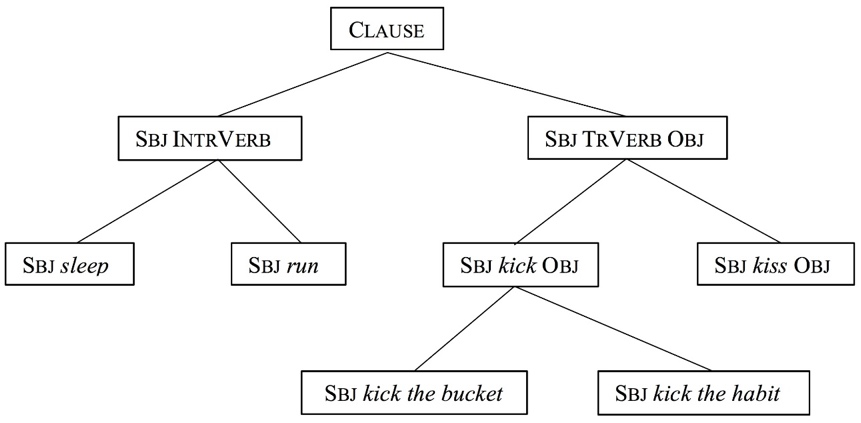
\includegraphics[width=\textwidth]{figures/a3-img001.jpg}
\caption{Taxonomic network of constructions (based on \citealt{CroftCruse2004}: 264)}
\label{fig:valdeson:1}

\begin{forest}
[\textsc{clause},rectangle,draw
	[\textsc{sbj} \textsc{intr} \textsc{verb}, rectangle, draw
		[\textsc{sbj} \textit{sleep},rectangle,draw
		]
		[\textsc{sbj} \textit{run},rectangle, draw
		]
	]
	[\textsc{sbj} \textsc{tr} \textsc{verb} \textsc{obj},rectangle, draw
		[
		\textsc{sbj} \textit{kick} \textsc{obj},rectangle, draw 
			[
			\textsc{sbj} \textit{kick the bucket},rectangle, draw
			]
			[
			\textsc{sbj} \textit{kick the habit},rectangle, draw
			]
		]
		[\textsc{sbj} \textit{kiss} \textsc{obj},rectangle, draw
		]
	]
]
\end{forest}
\end{figure}


\figref{fig:valdeson:1} illustrates the intransitive and transitive constructions in \ili{English}, with the schematic argument structure constructions on the second-highest level, below the clause level. The level below the \isi{argument structure construction} constitutes the same construction but with the verb slot filled. Knowledge about the use of a certain verb in a certain construction may be stored both at the schematic level and at the verb-specific level. \citet[25]{Croft2001} refers to the constructions in which the verb slot is filled as \textit{verb-specific constructions}. This notion of verb-specific constructions is highly relevant for the present study, as my object of study is the fourteen most common such verb-specific constructions that instantiate the more schematic \isi{double object construction}. Taking the network illustrated in \figref{fig:valdeson:1} as a starting point, the idea is that when the verb \textit{kick} is used in the transitive construction, it inherits properties from the general, superordinate transitive construction. However, the verb-specific transitive construction with \textit{kick} may at the same time contain idiosyncratic properties not inherited from the general transitive construction. This becomes even clearer when we look at an expression like \textit{kick the bucket}, which is linked to the verb-specific transitive construction with \textit{kick}, but at the same time carries the idiosyncratic non-compositional meaning ‘die’. While sharing properties with the superordinate level in the \isi{taxonomic hierarchy}, any idiosyncratic information stored at a lower level in the network overrides the more general information stored at a higher level (see \citealt{KemmerBarlow2000}: ix–x).


\subsection{Productivity}\label{sec:valdeson:3.2}


As will become clear, the results of the present study can readily be discussed in terms of constructional \isi{productivity}. The notion of \isi{productivity} refers to the ability of a construction to attract new types and is usually considered to be correlated with \isi{type frequency} in one way or another. At its most basic level, \isi{productivity} can be seen as directly correlated with the \isi{type frequency} of the construction (see e.g. \citealt{Bybee2010}). Applying this definition to an argument structure like the \isi{double object construction} implies that the \isi{productivity} of the construction can be estimated from the number of individual verbs occurring in the construction within a corpus.



In this study, I take the measure of \isi{lexical variation} (i.e. a \isi{type frequency} measure relative to the number of tokens) as an indication of \isi{productivity}. Since I focus mainly on the \isi{lexical variation} of direct objects in verb-specific constructions, the present study makes it possible to compare the \isi{productivity} of these verb-specific constructions over time, as well as between the constructions themselves.



In the model of \isi{productivity} presented by \textcite{Bardal2008} and  \citet{BardalGildea2015}, \isi{productivity} is regarded as a combination of the \isi{type frequency} and the semantic coherence of the construction. According to this model, a \isi{productive} construction is usually characterized by either a large \isi{type frequency} and a low degree of semantic coherence, or by a smaller \isi{type frequency} and a larger degree of semantic coherence. The present study does not offer a fully-fledged analysis of the semantics of the verb-specific constructions involved. Nonetheless, the topic is repeatedly made relevant in the presentation of the results, as several of the verb-specific constructions show a pattern in which a change in the direction of reduced \isi{lexical variation} is cotemporal with a shift towards the \isi{semantic specialization} of the \isi{direct object slot}, with this slot becoming increasingly associated solely with abstract direct objects.



The next section gives an account of the quantitative method employed in the study.


\subsection{Method}\label{sec:valdeson:3.3}


As already mentioned, one of the aims of the present study is to gain a better understanding of the \isi{productivity} of some of the verb-specific constructions within the DOC. As stated in \sectref{sec:valdeson:3.2} above, the \isi{productivity} of argument structure constructions is usually considered to be indicated, in one way or another, by the \isi{type frequency} of the verb slot. If we move one step down in the taxonomic construction hierarchy, the \isi{productivity} of verb-specific constructions can then, accordingly, be calculated by measuring the \isi{type frequency} of the \isi{direct object slot}.


\begin{sloppypar}
While measuring the \isi{type frequency} of a construction simply in absolute terms will render an accurate account of the actual \isi{type frequency} of a specific corpus, it does not allow for comparison across corpora and is thus not a fully appropriate measure if we want to investigate diachronic change. A more reasonable way of measuring \isi{type frequency} is to do it by means of the \isi{type-to-token ratio}. Traditionally, this method works at the text level by measuring the quotient of individual types divided by the total number of tokens in the text. This method of measurement has often been employed in language \isi{acquisition} studies, where a high \isi{type-to-token ratio} is seen as indicative of a more highly developed language (see e.g. the overview in \citealt{Richards1987}). It can be applied, however, to all tokens of a particular construction, rather than to all tokens in an entire text. The \isi{type-to-token ratio} of a construction is then measured as the quotient of the number of individual types divided by the total number of instances of the construction (see e.g. \citealt{Olofsson2019}).
\end{sloppypar}



While superior to measures of absolute frequency, the \isi{type-to-token ratio} is still marred by a certain inaccuracy when applied to texts or corpora of greatly varying size. Since the number of new individual types decreases the longer the text or corpus is, the \isi{type-to-token ratio} will normally be lower for a longer text than for a shorter one. This flaw can be counterbalanced by extracting samples of similar size from the texts measured (see e.g. \citealt{Baayen2008}: 223–226; \citealt{CovingtonMcFall2010}).



The method employed in the present study is an adaptation of the \isi{type-to-token ratio} that works on samples of equal size from all corpora. This procedure is often referred to as standardized \isi{type-to-token ratio} (see \citealt{McEneryHardie2012}: 50), but in the present paper I will refer to this measure simply as \textit{lexical variation}. For the DOC as a whole, the \isi{lexical variation} (i.e. the variation in the verb slot) was measured by extracting ten random samples of 1,000 tokens from each of the three time periods that the diachronic study encompasses. The samples were created using the RAND function in Excel. For each of these samples, I counted the number of individual verb lemmas. The actual \isi{lexical variation} is then taken to be the mean value of these ten samples. A similar procedure was undertaken for each of the fourteen verb-specific constructions studied, where the \isi{lexical variation} of the \isi{direct object slot} is in focus. For the verb-specific constructions, the samples varied in size between 20 and 100, depending on the lowest number of occurrences of the verb in \isi{question} found in one of the corpora. Thus, for example, if a verb occurs 25 times in the first period, 40 times in the second and 150 times in the third period, ten random samples of 20 occurrences are drawn from each period. In each sample, the individual number of noun lemmas in the \isi{direct object slot} was counted. Pronominal direct objects were not included in the study.



In order to obtain a comparable measure of \isi{lexical variation} across the verb-specific constructions, it is given as a percentage, with 100\% entailing the maximum level of \isi{lexical variation} with each token consisting of an individual type. The sample size varies according to the number of occurrences of the verb in \isi{question} in the subcorpora but is always set to a round number (20, 30, 40, 50, etc.). For each verb, the largest sample possible was used. A problem with this procedure is that the sample size differs between verbs, making it difficult to conduct a fully-fledged comparison between the different verb-specific constructions. More importantly, however, the method applied in the present study makes it possible to study the diachronic changes in \isi{lexical variation} for each \isi{verb-specific construction} individually across the three time periods. Subsequently, it is possible to compare the tendencies found with each \isi{verb-specific construction}, i.e. whether the \isi{lexical variation} increases, decreases, or remains relatively stable.



The other two frequency measures in the study are, perhaps, somewhat more straightforward. As mentioned in the introduction (\sectref{sec:valdeson:1}), I apply the term \textit{text frequency} to the normalized measure of occurrences per one million tokens. A similar \isi{frequency measure} is employed by \citet{Colleman2015} in a study of the \ili{Dutch} \textit{krijgen} \isi{passive} construction. Finally, I also look at the frequency of the most common verbs in the DOC relative to the total number of instances of the construction. For lack of a better term, I refer to this as \textit{verb frequency relative to construction}.


\section{Data}\label{sec:valdeson:4}


The present study is based on corpus data from various corpora from 1800 to 1999. All corpora consist mainly of prose fiction, making them comparable over time. The 19\textsuperscript{th} century data are taken from the \isi{SPF corpus} of \ili{Swedish} prose fiction 1800–1900 (available in \isi{Korp}, \citealt{BorinEtAl2012}), from which I extracted data from two timespans: 1800–1844 and 1898–1901.\footnote{\url{https://spraakbanken.gu.se/korp}}  The \isi{SPF corpus} contains \ili{Swedish} prose fiction data from the years 1800, 1820 etc. with continuing twenty-year intervals (including data from a few novels published in the years before or after the year in \isi{question}). As the amount of data from the years 1800 and 1820 is highly limited, the data from the early 19\textsuperscript{th} century cover a larger timespan than the data from the turn of the 20\textsuperscript{th} century. The present-day \ili{Swedish} data were gathered from three different corpora: \textit{Bonniersromaner I} (1976–1977), \textit{Bonniersromaner II} (1980–1981) and \textit{Norstedtsromaner} (1999). All the corpora were searched using the corpus infrastructure \isi{Korp} \citep{BorinEtAl2012}. Information about the corpora is summarized in \tabref{tab:valdeson:2}.


\begin{table}
\caption{The corpora\label{tab:valdeson:2}}
\begin{tabular}{llr}
\lsptoprule
Corpus & Timespan & No. tokens\\
\midrule
\textit{Svensk prosafiktion} (‘\ili{Swedish} prose fiction') & 1800–1844 & 2\,203\,451\\
\textit{Svensk prosafiktion} (‘\ili{Swedish} prose fiction') & 1898–1901 & 9\,837\,169\\
\textit{Bonniersromaner I} (‘Bonnier novels I’) & 1976–1977 & 6\,578\,450\\
\textit{Bonniersromaner II}  (‘Bonnier novels II’) & 1980–1981 & 4\,304\,271\\
\textit{Norstedtsromaner}  (‘Norstedts novels’) & 1999 & 2\,533\,209\\
\midrule
Total & 1800–1999 & 25\,456\,350\\
\lspbottomrule
\end{tabular}
\end{table}

In order to obtain a representative and sufficiently large amount of data, I searched the corpora using a search string designed to capture as many relevant results of the DOC as possible. For this, I employed the automatic part-of-speech tagger in \isi{Korp}. This tagger is trained on present-day \ili{Swedish} data, but studies within computer linguistics have shown that it works with an accuracy of almost 90\% even as far back as 18\textsuperscript{th} century \ili{Swedish} (see \citealt{AdesamEtAl2016}: 76). Considering this, there is no reason to doubt that the part-of-speech tagger is an efficient tool also for the 19\textsuperscript{th} century corpora. The search string (which is illustrated in \tabref{fig:valdeson:2}) was designed to capture all occurrences in the corpora of a verb followed by any personal pronoun in the \isi{object case}, followed by three random words that are neither verbs nor prepositions, and with a noun as its final element.



The search method restricts the data to instances of the DOC with a pronominal \isi{indirect object} and a full NP \isi{direct object}. Limiting the search string to pronominal indirect objects leads to higher precision, i.e. the search does not generate too much noise. While at the same time this comes at the expense of lower recall, i.e. the search method limits the amount of data I can acquire, the method acknowledges the often reported fact from studies on the \ili{English} \isi{double object construction} that the prototypical \isi{indirect object} is likely to be pronominal and to have an animate referent (see \citealt{BresnanEtAl2007}; see also \citealt{CollemanDe_Clerck2011} for the use of a similar method in a diachronic study of the \ili{English} \isi{double object construction}). This generalization most likely holds for \ili{Swedish} as well (see \citealt{TelemanEtAl1999}/3: 315, who confirm that the \isi{indirect object} in the \ili{Swedish} DOC most often has an animate referent). Collecting instances of the DOC with direct objects consisting of full noun phrases only is also a prerequisite for the method employed in the study, since the verb-specific constructions are studied with regard to the \isi{lexical variation} in the \isi{direct object slot}. I excluded all instances of \isi{reflexive} indirect objects, e.g. \textit{köpa sig ngt} ‘buy something for oneself’. \isi{Reflexive} indirect objects are extremely common in the \ili{Swedish} DOC, especially with verbs of creation (see \citealt{TelemanEtAl1999}/3: 317), and might be considered a construction in their own right, being subject to their own semantic and pragmatic constraints (cf. the treatment by Barðdal et al. 2011 of a similar construction in \ili{Norwegian}). The three random words between the pronoun in the \isi{object case} and the full noun allows space for attributes and articles preceding the head of the \isi{noun phrase} that constitutes the \isi{direct object}. Finally, the data set was manually checked, and all irrelevant hits were excluded.



\begin{table}
\begin{tabularx}{\textwidth}{lQQl}
\lsptoprule
Part of speech & Word & Word & Part of speech\\
\midrule
Verb & \textit{mig} ‘me’

\textit{dig} ‘you’ (\textsc{obj}.\textsc{sg})

\textit{henne} ‘her’

\textit{honom} ‘him’

\textit{oss} ‘us’

\textit{er} ‘you’ (\textsc{obj}.\textsc{pl})

\textit{eder} ‘you’ (\textsc{obj}.\textsc{pl})

\textit{dem} ‘them’ & <any word except prepositions and verbs>

<repeated 0–3 times> & Noun\\
\lspbottomrule
\end{tabularx}
\caption{Search string}
\label{fig:valdeson:2}
\end{table}


I divided the data into three periods – early 19\textsuperscript{th} century \ili{Swedish} (P1), turn-of-the-century \ili{Swedish} (P2) and present-day \ili{Swedish} (P3). The \isi{periodization} is illustrated in \tabref{tab:valdeson:3}, which also gives information on the number of instances of the DOC retrieved for each period.


\begin{table}
\caption{The data}
\label{tab:valdeson:3}
\begin{tabular}{lrr}
\lsptoprule
Period & Corpus size & DOC instances\\
\midrule
P1 (1800–1844) & 2\,203\,451 & 1\,850\\
P2 (1898–1901) & 9\,837\,169 & 6\,798\\
P3 (1976–1999) & 13\,415\,930 & 5\,871\\
\midrule
Total & 25\,456\,350 & 14\,519\\
\lspbottomrule
\end{tabular}
\end{table}

\section{Results}\label{sec:valdeson:5}


In this section I present the results of the study. \sectref{sec:valdeson:5.1} gives an overview of the DOC as a whole, while \sectref{sec:valdeson:5.2} zooms in on the verb-specific tendencies. The verb-specific constructions are then treated in detail in \sectref{sec:valdeson:5.3}, where the individual verbs are discussed one by one.


\subsection{General overview of the double object construction}\label{sec:valdeson:5.1}


As \tabref{tab:valdeson:4} illustrates, the \isi{lexical variation} in the verb slot in the \ili{Swedish} DOC has been gradually decreasing over the last 200 years, with the \isi{lexical variation} dropping around three percentage points between each measuring point, from 13.2\% in P1 to 7.7\% in P3. In plain language, this means that out of 1,000 random occurrences of the DOC in early 19\textsuperscript{th} century prose fiction \ili{Swedish}, 132 individual verb types can be found. A similar sample of 1,000 tokens in present-day \ili{Swedish} prose fiction renders only 77 individual verb types. This indicates that the DOC has become more specified in present-day \ili{Swedish}, as the construction seems to be compatible with a more limited number of verbs. This narrowing of the \isi{lexical variation} is paralleled by both a decrease in the \isi{text frequency} of the DOC and a \isi{semantic specialization} over time, as shown in \textcite{ValdesonSubmitted}.


\begin{table}
\caption{Lexical variation of verbs in the DOC}
\label{tab:valdeson:4}
\begin{tabular}{lrr}
\lsptoprule
Period & Types per 1,000 tokens & \isi{Lexical variation}\\
\midrule
1800–1844 & 132 & 13.2\%\\
1898–1901 & 108 & 10.8\%\\
1976–1999 & 77 & 7.7\%\\
\lspbottomrule
\end{tabular}
\end{table}

One aspect that clearly correlates with the decreased \isi{lexical variation} of the DOC is the rise in \isi{relative frequency} of the verb \textit{ge} ‘give’ within the construction. This verb constitutes around 20\% of all occurrences of the DOC in P1. In P3, the share has increased to almost 60\%. This means that more than half of the occurrences of the DOC in present-day \ili{Swedish} are instances of the verb \textit{ge}. With one single verb being so dominant, it is of course more difficult to achieve a high \isi{lexical variation}. \tabref{tab:valdeson:5} gives an overview of the ten most common verbs in the DOC in each of the three periods. The verbs appearing on the list in all three periods are printed in boldface in the table. These fourteen verbs were selected as the object of study for the investigation of \isi{lexical variation} in the \isi{direct object slot} of verb-specific constructions. Since the measure of \isi{lexical variation} introduced in this paper concerns the \isi{lexical variation} in the \isi{direct object slot}, it is of importance that the verb-specific constructions studied are frequent enough across all three subcorpora for any quantitative changes to be discerned.

\begin{table}
\caption{Top ten verbs in each period\label{tab:valdeson:5}}
\begin{subtable}{.5\linewidth}\centering
\caption{P1 (1800–1844)}
\begin{tabularx}{\linewidth}{Xrr}
\lsptoprule
Verb & Abs.   & Rel.   \\
\midrule
\textbf{\textit{ge}} ‘give’             & 369 & 19.9\%    \\
\textbf{\textit{göra}} ‘make, do’       & 188 & 10.2\%    \\
\textbf{\textit{visa}} ‘show’           & 109 & 5.9\%     \\
\textit{lämna} ‘hand’                   & 106 & 5.7\%     \\
\textbf{\textit{räcka}} ‘hand’          & 75 & 4.1\%      \\
\textbf{\textit{skänka}} ‘give’         & 73 & 3.9\%      \\
\textbf{\textit{säga}} ‘say, tell’      & 65 & 3.5\%      \\
\textbf{\textit{skaffa}} ‘obtain’       & 46 & 2.5\%      \\
\textit{kosta} ‘cost’                   & 33 & 1.8\%      \\
\textit{skicka} ‘send’                  & 29 & 1.6\%      \\
(…) & (…) & (…) \\
\midrule
Total & 1,850 & 100.0\%  \\
\lspbottomrule
\end{tabularx}
\end{subtable}\begin{subtable}{.5\linewidth}\centering
\caption{P2 (1898–1901)}
\begin{tabularx}{\linewidth}{Xrr}
\lsptoprule
Verb & Abs.   & Rel.   \\
\midrule
 \textbf{\textit{ge}} ‘give’         & 1\,852 & 27.2\%    \\
 \textbf{\textit{göra}} ‘make, do’   & 505 & 7.4\%       \\
 \textbf{\textit{räcka}} ‘hand’      & 343 & 5.0\%       \\
 \textbf{\textit{visa}} ‘show’       & 336 & 4.9\%       \\
 \textit{lämna} ‘hand’               & 290 & 4.3\%       \\
 \textbf{\textit{säga}} ‘say, tell’  & 255 & 3.8\%       \\
 \textbf{\textit{skänka}} ‘give’    & 247 & 3.6\%        \\
 \textbf{\textit{skaffa}} ‘obtain’   & 195 & 2.9\%       \\
 \textit{bereda} ‘cause’            & 194 & 2.9\%        \\
 \textit{beröva} ‘deprive’           & 118 & 1.7\%       \\
(…) & (…) & (…) \\
 \midrule
 Total & 6\,798 & 100.0\%\\
\lspbottomrule
\end{tabularx}
\end{subtable}\begin{subtable}{.5\linewidth}
\caption{P3 (1976–1999)}
\begin{tabularx}{\linewidth}{Xrr}
    \lsptoprule
Verb & Abs.   & Rel.   \\
\midrule
\textbf{\textit{ge}} ‘give’ & 3\,390 & 57.7\%\\
 \textbf{\textit{visa}} ‘show’ & 346 & 5.9\%\\
 \textbf{\textit{räcka}} ‘hand’ & 252 & 4.3\%\\
 \textbf{\textit{göra}} ‘make, do’ & 181 & 3.1\%\\
 \textit{erbjuda} ‘offer’           & 115 & 2.0\%\\
 \textbf{\textit{skänka}} ‘give’ & 103 & 1.8\%\\
 \textit{inge} ‘infuse’ & 86 & 1.5\%\\
 \textbf{\textit{skaffa}} ‘obtain’ & 86 & 1.5\%\\
 \textbf{\textit{säga}} ‘say, tell’ & 79 & 1.3\%\\
 \textit{skicka} ‘send’ & 69 & 1.2\%\\
(…) & (…) & (…) \\
 \midrule
 Total & 5\,871 & 100.0\%\\
\lspbottomrule
\end{tabularx}
\end{subtable}
\end{table}



% \begin{table}
% \caption{Top ten verbs in each period}
% \label{tab:valdeson:5}
% \fittable{
% \begin{tabular}{l@{}rrl@{}rrl@{}rr}
% \lsptoprule
% \multicolumn{3}{c}{P1 (1800–1844)} & \multicolumn{3}{c}{P2 (1898–1901)} & \multicolumn{3}{c}{P3 (1976–1999)}\\
% Verb & Abs. freq. & Rel. freq. & Verb & Abs. freq. & Rel. freq. & Verb & Abs. freq. & Rel. freq.\\
% \textbf{\textit{ge}} ‘give’ & 369 & 19.9\% & \textbf{\textit{ge}} ‘give’ & 1,852 & 27.2\% & \textbf{\textit{ge}} ‘give’ & 3,390 & 57.7\%\\
% \textbf{\textit{göra}} ‘make, do’ & 188 & 10.2\% & \textbf{\textit{göra}} ‘make, do’ & 505 & 7.4\% & \textbf{\textit{visa}} ‘show’ & 346 & 5.9\%\\
% \textbf{\textit{visa}} ‘show’ & 109 & 5.9\% & \textbf{\textit{räcka}} ‘hand’ & 343 & 5.0\% & \textbf{\textit{räcka}} ‘hand’ & 252 & 4.3\%\\
% \textit{lämna} ‘hand’ & 106 & 5.7\% & \textbf{\textit{visa}} ‘show’ & 336 & 4.9\% & \textbf{\textit{göra}} ‘make, do’ & 181 & 3.1\%\\
% \textbf{\textit{räcka}} ‘hand’ & 75 & 4.1\% & \textit{lämna} ‘hand’ & 290 & 4.3\% & \textit{erbjuda} ‘offer’ & 115 & 2.0\%\\
% \textbf{\textit{skänka}} ‘give’ & 73 & 3.9\% & \textbf{\textit{säga}} ‘say, tell’ & 255 & 3.8\% & \textbf{\textit{skänka}} ‘give’ & 103 & 1.8\%\\
% \textbf{\textit{säga}} ‘say, tell’ & 65 & 3.5\% & \textbf{\textit{skänka}} ‘give’ & 247 & 3.6\% & \textit{inge} ‘infuse’ & 86 & 1.5\%\\
% \textbf{\textit{skaffa}} ‘obtain’ & 46 & 2.5\% & \textbf{\textit{skaffa}} ‘obtain’ & 195 & 2.9\% & \textbf{\textit{skaffa}} ‘obtain’ & 86 & 1.5\%\\
% \textit{kosta} ‘cost’ & 33 & 1.8\% & \textit{bereda} ‘cause’ & 194 & 2.9\% & \textbf{\textit{säga}} ‘say, tell’ & 79 & 1.3\%\\
% \textit{skicka} ‘send’ & 29 & 1.6\% & \textit{beröva} ‘deprive’ & 118 & 1.7\% & \textit{skicka} ‘send’ & 69 & 1.2\%\\
% (…) & (…) & (…) & (…) & (…) & (…) & (…) & (…) & (…)\\
% Total & 1,850 & 100.0\% & Total & 6,798 & 100.0\% & Total & 5,871 & 100.0\%\\
% \lspbottomrule
% \end{tabular}
% }
% \end{table}

The verbs in the table pertain to a number of different semantic categories, including \isi{transfer} (\textit{ge} ‘give’, \textit{räcka} ‘hand’), communication (\textit{säga} ‘say, tell’, \textit{visa} ‘show’), and dispossession (\textit{beröva} ‘deprive’, \textit{kosta} ‘cost’). I make no principled distinction between verbs for which the presence of an \isi{indirect object} might be argued to be due to the \isi{valency} of the verb, like \textit{ge} ‘give’ and \textit{kosta} ‘cost’, and verbs construed with what is often referred to as a free \isi{dative} (or free \isi{indirect object}), like \textit{göra} ‘make, do’ (e.g. \textit{göra ngn ett par stövlar} ‘make sb. a pair of boots’) and \textit{skaffa} ‘obtain’ (e.g. \textit{skaffa ngn ett hus} ‘obtain a house for sb.’). This is in line with studies on argument structure constructions from a \isi{construction grammar} perspective, where the focus tends to be on the syntactic and semantic nature of the construction rather than the \isi{valency} of the verb (see \citealt{Goldberg1995}). Furthermore, the fact that a verb occurs frequently in the DOC indicates that the presence of an \isi{indirect object} is more likely to be a part of the lexical behaviour of the verb. For example, \citet[150--151]{Nielsen2019} discusses the fact that the \ili{Danish} verb \textit{skaffe} ‘obtain’, which is usually not claimed to occur with a valency-governed \isi{indirect object}, has properties that make it similar to verbs that are lexically \isi{ditransitive}.


\subsection{Overview of verb-specific tendencies}\label{sec:valdeson:5.2}


The use of the fourteen verb-specific constructions was investigated in three different ways: \isi{relative frequency} (out of all instances of the DOC), \isi{text frequency}, and \isi{lexical variation}. The \isi{relative frequency} is shown in \tabref{tab:valdeson:5} in the preceding section. \tabref{tab:valdeson:6} below presents the diachronic developments in \isi{text frequency} for each of the fourteen verb-specific constructions. The table shows how many times the \isi{verb-specific DOC} in \isi{question} occurs per one million corpus tokens. The figures are thus not relative to the total number of instances of the DOC. It is worth noting, however, that, as shown in \tabref{tab:valdeson:1} (in \sectref{sec:valdeson:2}), the \isi{text frequency} of the construction as a whole is reduced by almost half, from 840 occurrences per one million tokens in P1 to 445 occurrences per one million tokens in P3. Considering this general tendency, the expected outcome for each \isi{verb-specific construction} would be a similar decrease in \isi{text frequency}. Any development in any other direction, or of another magnitude, thus indicates that the use of the \isi{verb-specific construction} is changing in its own direction.



\tabref{tab:valdeson:6} shows the number of occurrences per one million corpus tokens of the fourteen verb-specific constructions (i.e. the number of occurrences of the verb used in the DOC). The figures in \tabref{tab:valdeson:6} clearly indicate that most verb-specific constructions are on the decrease. Some, like \textit{kosta} ‘cost’ and \textit{visa} ‘show’, are decreasing in use at roughly the same pace as the DOC in general, while others, like \textit{göra} ‘make, do’ and \textit{lämna} ‘hand’, manifest more dramatic drops. The only \isi{verb-specific construction} that increases in use is the DOC with \textit{ge} ‘give’, which has a \isi{text frequency} going up from 168 to 253 occurrences per one million words. A conclusion that can be drawn from this is that the increase in \isi{relative frequency} of \textit{ge} that was revealed in the previous section is not just due to the other verbs becoming less common, but also to the fact that the use of \textit{ge} has increased immensely, in stark contrast to the DOC as a whole.


\begin{table}
\caption{Occurrences of the verb-specific DOCs per million corpus tokens}
\label{tab:valdeson:6}
\begin{tabularx}{.9\textwidth}{lrrr}
\lsptoprule
Verb & P1 (1800–1844) & P2 (1898–1901) & P3 (1976–1999)\\
\midrule
\textit{bereda} ‘cause’ & 12.7 & 19.7 & 2.8\\
\textit{beröva} ‘deprive’ & 12.3 & 12.0 & 2.0\\
\textit{erbjuda} ‘offer’ & 9.5 & 6.1 & 8.6\\
\textit{ge} ‘give’ & 167.5 & 188.3 & 252.7\\
\textit{göra} ‘make, do’ & 85.3 & 51.3 & 13.5\\
\textit{inge} ‘infuse’ & 10.9 & 8.5 & 6.4\\
\textit{kosta} ‘cost’ & 15.0 & 11.7 & 5.1\\
\textit{lämna} ‘hand’ & 48.1 & 29.5 & 3.1\\
\textit{räcka} ‘hand’ & 34.0 & 34.9 & 18.8\\
\textit{skaffa} ‘obtain’ & 20.9 & 19.9 & 6.4\\
\textit{skicka} ‘send’ & 13.2 & 6.0 & 5.1\\
\textit{skänka} ‘give’ & 33.1 & 25.1 & 7.7\\
\textit{säga} ‘say, tell’ & 29.5 & 25.9 & 5.9\\
\textit{visa} ‘show’ & 49.5 & 34.2 & 25.8\\
\lspbottomrule
\end{tabularx}
\end{table}

Finally, \tabref{tab:valdeson:7} shows the \isi{lexical variation} in the \isi{direct object slot} for the fourteen verb-specific constructions, i.e., a standardized type-token ratio rendered as a percentage figure, where 100\% means that all occurrences of the \isi{verb-specific construction} in \isi{question} have different nouns as their \isi{direct object}. What counts as the \isi{direct object} here is the lemma form of the noun constituting the head of the \isi{noun phrase} that forms the \isi{direct object}. To explain how the figures in \tabref{tab:valdeson:7} were arrived at, we can use the verb \textit{bereda} as an example. Ten random samples of 20 occurrences each were created for the verb in each of the three periods. The mean value of the individual number of noun lemmas in the \isi{direct object slot} was then divided by 20 (i.e., the sample size), which provided the percentage figures presented in \tabref{tab:valdeson:7}. \sectref{sec:valdeson:5.3} below presents a more detailed account of each \isi{verb-specific construction}.



The figures presented in \tabref{tab:valdeson:7} indicate that there is a general tendency towards a lower rather than higher \isi{lexical variation} in the \isi{direct object slot} of the verb-specific constructions, with the most dramatic drops seen with the verbs \textit{bereda} ‘cause’, \textit{beröva} ‘deprive’, \textit{göra} ‘make, do’ and \textit{lämna} ‘hand’. However, most verbs show a relatively stable \isi{lexical variation}, with two verbs even undergoing an increase in \isi{lexical variation} (somewhat surprisingly) – \textit{räcka} ‘hand’ and \textit{visa} ‘show’.


\begin{table}
\caption{Lexical variation of direct objects in the verb-specific DOCs}
\label{tab:valdeson:7}
\begin{tabularx}{.9\textwidth}{lrrr}
\lsptoprule
Verb & P1 (1800–1844) & P2 (1898–1901) & P3 (1976–1999)\\
\midrule
\textit{bereda} ‘cause’ & 84.5\% & 68.0\% & 54.5\%\\
\textit{beröva} ‘deprive’ & 89.0\% & 83.5\% & 94.5\%\\
\textit{erbjuda} ‘offer’ & 95.5\% & 85.5\% & 94.5\%\\
\textit{ge} ‘give’ & 77.4\% & 77.0\% & 83.0\%\\
\textit{göra} ‘make, do’ & 41.7\% & 33.0\% & 16.2\%\\
\textit{inge} ‘infuse’ & 71.0\% & 61.5\% & 76.5\%\\
\textit{kosta} ‘cost’ & 67.0\% & 58.7\% & 72.3\%\\
\textit{lämna} ‘hand’ & 88.0\% & 67.5\% & 69.5\%\\
\textit{räcka} ‘hand’ & 22.4\% & 38.2\% & 70.6\%\\
\textit{skaffa} ‘obtain’ & 94.0\% & 89.8\% & 85.0\%\\
\textit{skicka} ‘send’ & 94.0\% & 94.0\% & 89.5\%\\
\textit{skänka} ‘give’ & 81.0\% & 77.2\% & 89.2\%\\
\textit{säga} ‘say, tell’ & 53.6\% & 35.8\% & 14.6\%\\
\textit{visa} ‘show’ & 64.8\% & 62.7\% & 79.5\%\\
\lspbottomrule
\end{tabularx}
\end{table}

In the next section, I will go through the fourteen verbs one by one and give a more detailed account of the tendencies already observed in the current section.


\subsection{Lexical variation of direct objects in fourteen verb-specific constructions}\label{sec:valdeson:5.3}


The fourteen verbs investigated in the study can conveniently be divided into three groups based on whether they show a type-token ratio for direct objects that is decreasing (these verbs are dealt with in \sectref{sec:valdeson:5.3.1}), increasing (\sectref{sec:valdeson:5.3.2}), or relatively stable (\sectref{sec:valdeson:5.3.3}). For the sake of convenience, a decrease or increase in type-token ratio has been arbitrarily defined as a change of at least ten percentage points between P1 and P3.\footnote{A reviewer remarks that it is somewhat problematic that the three periods P1–P3 are of unequal length. The data were collected with the intention of retrieving data from the early 19\textsuperscript{th} century, the turn of the 20\textsuperscript{th} century, and the late 20\textsuperscript{th} century. As mentioned in \sectref{sec:valdeson:4} above, the first period covers a larger time span than the other periods due to the fact that there is not much available data from the 19\textsuperscript{th} century prior to 1840. Similarly, due to the fact that the DOC is relatively infrequent in present-day \ili{Swedish}, I considered it preferable to collect as much data as possible from the end of the 20\textsuperscript{th} century, in order to conduct the kind of quantitative analyses presented in this paper.}  The highly frequent verb \textit{ge} ‘give’ undergoes a development that evidently deviates from all other verbs in the DOC. For this reason, \textit{ge} ‘give’ is dealt with separately in \sectref{sec:valdeson:5.3.4}.


\subsubsection{Verb-specific constructions undergoing a decrease in lexical variation in the direct object slot}\label{sec:valdeson:5.3.1}


Four verb-specific constructions in my study display a decrease of ten percentage points or more in their \isi{lexical variation}. These verbs are \textit{bereda} ‘cause’, \textit{göra} ‘make, do’, \textit{lämna} ‘hand’, and \textit{säga} ‘say, tell’. For all four, this decrease is accompanied by a reduced use of the verb in the DOC overall.



\subsubsubsection{\textit{bereda} ‘cause’}\label{sec:valdeson:5.3.1.1}





The verb \textit{bereda} (which is translated here as ‘cause’, but which can also be used for meanings such as ‘prepare’ and, simply, ‘give’) constitutes one of the least frequent verb-specific constructions in the study. As \tabref{tab:valdeson:8} shows, the verb is not just infrequent when used in the DOC, but is a rather infrequent verb overall. It displays a rather dramatic drop in \isi{lexical variation}, decreasing from 85\% in P1 to 55\% in P3. This indicates that it was used with a much wider range of direct objects in the early 19\textsuperscript{th} century than is the case in present-day \ili{Swedish}. As expected, the decreased variation in direct objects with \textit{bereda} is accompanied by a general decrease in \isi{text frequency} of the \isi{verb-specific construction} from P1 to P3. However, while the decrease in \isi{lexical variation} appears to constitute a gradual change from the early 19\textsuperscript{th} century onwards, the drop in \isi{text frequency} does not occur until the 20\textsuperscript{th} century. In fact, the \isi{verb-specific construction} sees a rather sharp increase in \isi{text frequency} between P1 and P2. These apparently conflicting tendencies indicate that there does not necessarily have to be a one-to-one correspondence between decreased \isi{lexical variation} and a decrease in \isi{text frequency}.


\begin{table}
\caption{Frequency measures of the verb-specific DOC with \textit{bereda} ‘cause’\label{tab:valdeson:8}}
\fittable{\begin{tabular}{lr@{ }rrrr@{ }r}
\lsptoprule
Period & \multicolumn{2}{c}{Freq. rel. to DOC} & \multicolumn{2}{c}{Occ./mil. tokens} & \multicolumn{2}{c}{Lexical variation}\\\cmidrule(lr){4-5}
&  &  & In general & In DOC &  & \\
\midrule
P1 (1800–1844) & 28/1\,850 & 1.5\%  & 96.2 & 12.7 & 16.9/20 & 84.5\%\\
P2 (1898–1901) & 194/6\,798 & 2.9\% & 111.3 & 19.7 & 13.6/20 & 68.0\%\\
P3 (1976–1999) & 37/5\,871 & 0.6\%  & 18.6 & 2.8 & 10.9/20 & 54.5\%\\
\lspbottomrule
\end{tabular}}
\end{table}

Interestingly, the changes in \isi{text frequency} of the \isi{verb-specific DOC} with \textit{bereda} are paralleled by the changes in \isi{text frequency} of the verb in general. This might at first glance seem unsurprising, but as the survey of verbs below reveals, there is not necessarily any apparent correlation between the observed changes in \isi{text frequency} for the verb in the DOC and the verb in general. The fact that such a correlation is found with the verb \textit{bereda} indicates that the decreased use of the \isi{verb-specific DOC} is the result of the verb generally losing popularity. Furthermore, the decrease in \isi{lexical variation} reveals a more stereotypical use of the verb in present-day \ili{Swedish} compared to the early 19\textsuperscript{th} century. In practice, this more restricted use of the verb in the DOC is manifested by a predominance in present-day \ili{Swedish} for the use of \textit{bereda} mainly with direct objects with abstract referents (usually denoting feelings and the like). In the 19\textsuperscript{th} century data, the verb also frequently occurs with concrete direct objects, something that is rarely seen in present-day \ili{Swedish}. (Note that this change could be analysed as a process of \isi{semantic narrowing} of the verb as such, in which the verb loses the ability to denote events of physical preparation while still retaining the notion of abstract \isi{causation}.) The example in \REF{ex:valdeson:8} below shows a 19\textsuperscript{th} century occurrence of \textit{bereda} with a concrete \isi{direct object}, while \REF{ex:valdeson:9} illustrates the modern usage, limited to mainly abstract direct objects, the most prominent ones being \textit{nöje} and \textit{glädje}, both carrying the meaning ‘joy’.\footnote{The noun phrases constituting the direct objects were not consistently tagged as concrete or abstract, i.e. these notions were not operationalized in any specific way. Consequently, the report on the use of the verb \textit{bereda} with concrete or abstract direct objects is based on the author’s impressionistic observations.}


\ea \label{ex:valdeson:8}
\gll Hindiah lät framsatta silfwerpannan   och tända eld, för att \textbf{\textit{bereda}} \textit{oss}  \textit{den} \textit{aromatiska}    \textit{kaffedryck},   \textit{som}  \textit{endast}  \textit{rätt}    \textit{kan}  \textit{tillagas} \textit{och}  \textit{njutas}      \textit{i}    \textit{sitt}  \textit{hemland},  \textit{Indien}. \\
   Hindiah let put\_forth  silver\_kettle:\textsc{def}     and light  fire for to prepare us    that  aromatic       coffee\_drink  which  only    rightly  can   be\_made and  be\_relished    in    its    homeland     India\\
\glt ‘Hindiah had the silver kettle put forth and a fire lit, in order to prepare us that aromatic coffee drink, which can only be rightly made and relished in its homeland, India’ (1800–1844)
\ex \label{ex:valdeson:9}
\gll Och  det    skulle \textbf{\textit{bereda}} \textit{mig}  \textit{det}  \textit{största}    \textit{nöje}!\\
  and      that      would  cause      me    the  greatest  pleasure\\
\glt `And that would bring me the greatest pleasure!’ (1976–1999)
\z


\subsubsubsection{\textit{göra} ‘make, do’}\label{sec:valdeson:5.3.1.2}



The verb \textit{göra} underwent some rather dramatic changes during the period investigated. It constituted the second most frequent \isi{verb-specific DOC} in P1 and P2, but experienced a continuing decrease in frequency relative to the DOC as a whole, as well as a rather drastic drop in \isi{text frequency} when used in the DOC. (The overall \isi{text frequency} of the verb, on the other hand, seems to be stable between P1 and P3, although a deviant peak in the usage is found in P2.) The \isi{verb-specific construction} with \textit{göra} has a relatively low \isi{lexical variation} in P1 (42\%), indicating that the verb was already used in the early 19\textsuperscript{th} century in a lot of \isi{fixed expressions} with \isi{ditransitive} syntax. This tendency becomes more and more pronounced over the course of time, and in P3 the \isi{lexical variation} is down to a mere 16\%.


\begin{table}
\caption{Frequency measures of the verb-specific DOC with \textit{göra} ‘make, do’\label{tab:valdeson:9}}
\fittable{\begin{tabular}{lr@{ }rrrr@{ }r}
\lsptoprule
Period & \multicolumn{2}{c}{Freq. rel. to DOC} & \multicolumn{2}{c}{Occ./mil. tokens} & \multicolumn{2}{c}{Lexical variation}\\\cmidrule(lr){4-5}
&  &  & In general & In DOC &  & \\
\midrule
P1 (1800–1844) & 188/1\,850 & 10.2\% & 2\,404.4 & 85.3 & 41.7/100 & 41.7\%\\
P2 (1898–1901) & 505/6\,798 & 7.4\% & 4\,170.6 & 51.3 & 33.0/100 & 33.0\%\\
P3 (1976–1999) & 181/5\,871 & 3.1\% & 2\,945.1 & 13.5 & 16.2/100 & 16.2\%\\
\lspbottomrule
\end{tabular}}
\end{table}

The tendencies identified for \textit{göra} correspond relatively closely to those found with the verb \textit{bereda} (see above). The verbs have similar semantics, both showing polysemy in that they can refer to concrete events of creation (in the case of \textit{göra}) or preparation (in the case of \textit{bereda}) as well as abstract events of \isi{causation}, where the \isi{direct object} typically refers to some kind of feeling or sensation. With both \textit{bereda} and \textit{göra}, the concrete use of the verbs in the DOC is infrequent (basically non-existent) in present-day \ili{Swedish}, whereas such examples can readily be found in the 19\textsuperscript{th} century data. This 19\textsuperscript{th} century concrete use of \textit{göra} in the DOC is illustrated in \REF{ex:valdeson:10}. When the verb is used in the DOC in present-day \ili{Swedish}, this is mainly with direct objects with an abstract reference. Most occurrences of the verb \textit{göra} in the DOC in present-day \ili{Swedish} are found in the \isi{fixed expressions} \textit{göra ngn sällskap} ‘keep someone company’ and \textit{göra ngn en tjänst} ‘do someone a favour’. However, other direct objects can still be found, as exemplified in \REF{ex:valdeson:11}.


\ea \label{ex:valdeson:10}
\gll I       har  en  gång \textbf{\textit{gjort}} \textit{mig}  \textit{ett} \textit{par} \textit{stöflar},  \textit{som}  \textit{klämt}   \textit{värre} än      om  de   varit  spanska.\\
  You    have    one   time  made  me  a    pair  boots    that  pinched worse than    if        they    been  \ili{Spanish} \\
\glt ‘You once made me a pair of boots that pinched worse than if they had been \ili{Spanish}.’ (1898–1901)
\ex \label{ex:valdeson:11}
\gll björnen  kommer  inte    mer      att \textbf{\textit{göra}} \textit{er}    \textit{någon}  \textit{skada}.\\
  bear:\textsc{def}         will        not  anymore     to  do      you  any     harm\\
\glt `the bear will not do you any harm anymore.’ (1976–1999)
\z


The range of abstract nouns that occur as the \isi{direct object} of \textit{göra} seems to be more limited in present-day \ili{Swedish} compared to 19\textsuperscript{th} century \ili{Swedish}. It seems reasonable to conclude that the verb \textit{göra} has lost two functions in the DOC – the ability to co-occur with concrete direct objects, and the function as a dummy/light verb together with a more substantial abstract \isi{direct object}. The first of these functions, the ability to occur with concrete objects, is still maintained in the prepositional alternative \textit{göra ngt åt ngn} ‘make something for someone’, whereas regarding the second function, the verb \textit{ge} ‘give’ has knocked out all other verbs as the main dummy verb in light verb constructions with verb\,+\,\isi{indirect object}\,+\,abstract \isi{direct object} (cf. \citealt{Sundquist2020} regarding a similar increase in the use of \textit{give} as a light verb in \ili{English} during the same period).



\subsubsubsection{\textit{lämna} ‘hand’}\label{sec:valdeson:5.3.1.3}



The verb \textit{lämna} ‘hand’ is quite often used more or less synonymously with \textit{ge} ‘give’, and occurs with direct objects denoting both concrete and abstract referents. As in the case of \textit{bereda} and \textit{göra}, the use of the verb with concrete objects seems to be diminishing, and this is most likely the main reason why the \isi{lexical variation} went down from 88\% in P1 to just under 70\% in P3. This tendency, however, is not as strong for \textit{lämna} as for \textit{bereda} and \textit{göra}, indicating that \textit{lämna} is not just used in a limited number of \isi{fixed expressions}. It is also interesting to note that the \isi{lexical variation} only decreased between P1 and P2, while it remained relatively stable throughout the 20\textsuperscript{th} century. What happened between P2 and P3, on the other hand, was a distinct decrease in \isi{text frequency}, accompanied by a sharp drop in the \isi{relative frequency} of the \isi{verb-specific DOC} in relation to the DOC as a whole. Taking both these tendencies into account, we find that the use of the \isi{verb-specific DOC} with \textit{lämna} is decreasing while the \isi{productivity} of the construction is still relatively intact.


\begin{table}
\caption{Frequency measures of the verb-specific DOC with \textit{lämna} ‘hand’\label{tab:valdeson:10}}
\fittable{\begin{tabular}{lr@{ }rrrr@{ }r}
\lsptoprule
Period & \multicolumn{2}{c}{Freq. rel. to DOC} & \multicolumn{2}{c}{Occ./mil. tokens} & \multicolumn{2}{c}{Lexical variation}\\\cmidrule(lr){4-5}
&  &  & In general & In DOC &  & \\
\midrule
P1 (1800–1844) & 106/1\,850 & 5.7\% & 565.0 & 48.1 & 35.2/40 & 88.0\%\\
P2 (1898–1901) & 290/6\,798 & 4.3\% & 960.4 & 29.5 & 27.0/40 & 67.5\%\\
P3 (1976–1999) & 41/5\,871 & 0.7\% & 409.2 & 3.1 & 27.8/40 & 69.5\%\\
\lspbottomrule
\end{tabular}}
\end{table}

The example in \REF{ex:valdeson:12} illustrates how \textit{lämna} is used with concrete objects in the 19\textsuperscript{th} century data. In \REF{ex:valdeson:13}, we see the typical use of \textit{lämna} in present-day \ili{Swedish}, i.e. with abstract direct objects. In present-day \ili{Swedish}‚ \textit{lämna} can often be replaced with \textit{ge} ‘give’, and this might have led to the verb \textit{ge} gaining ground at the expense of \textit{lämna}.


\ea \label{ex:valdeson:12}
\gll men kammarpigan   berättade  hans  svar     för     sin     fröken, hvilken leende \textbf{\textit{lemnade}} \textit{henne}  \textit{en}  \textit{flaska}    \textit{malörtsdroppar}\\
  but maid.\textsc{def}        told        his    answer  to  her   lady who       smiling    handed       her        a  bottle       wormwood\_tincture\\
\glt `but the maid told his answer to her lady, who smiling handed her a bottle of wormwood tincture’ (1800–1844)\\
\ex \label{ex:valdeson:13}
\gll en    iskall  närgången  vind   som    inte \textbf{\textit{lämnade}} \textit{henne}  \textit{någon}   \textit{ro}\\
  an   icy          intrusive     wind  that      not  gave      her   any  peace  \\
\glt `an icy creeping wind that didn’t give her any peace’ (1976–1999)
\z


\subsubsubsection{\textit{säga} ‘say, tell’}\label{sec:valdeson:5.3.1.4}\largerpage[-1]
One of the general changes in the \isi{semantic range} of the DOC identified in \textcite{ValdesonSubmitted} is the diminishing use of \isi{verbs of communication} in the DOC. This tendency is mainly reflected by the fact that several \isi{verbs of communication} have lost the ability to occur in the DOC in present-day \ili{Swedish}, among them the verb \textit{berätta} ‘tell’, which occurs relatively frequently in the construction in 19\textsuperscript{th} century \ili{Swedish}. A handful of \isi{communication verbs} are still found in the DOC in present-day \ili{Swedish}, but the use of the verb \textit{säga}, which is the most frequent verb denoting verbal communication, shows a decline in \isi{lexical variation} in the \isi{direct object slot}. The change in the behavior of the verb is roughly similar to that of \textit{göra} ‘make, do’. A shared feature of these verbs is that they are both common verbs in present-day \ili{Swedish} (unlike, for example, \textit{bereda}, which has a more old-fashioned tone). The fact that \textit{säga} is a common everyday verb in present-day \ili{Swedish} is not least indicated by the fact that the overall \isi{text frequency} of the verb has gone up markedly, from about 2,000 occurrences per one million tokens in the early 19\textsuperscript{th} century to 6,000 occurrences per one million tokens in present-day \ili{Swedish}.


\begin{table}
\caption{Frequency measures of the verb-specific DOC with \textit{säga} ‘say, tell’}
\label{tab:valdeson:11}
\fittable{\begin{tabular}{lr@{ }rrrr@{ }r}
\lsptoprule
Period & \multicolumn{2}{c}{Freq. rel. to DOC} & \multicolumn{2}{c}{Occ./mil. tokens} & \multicolumn{2}{c}{Lexical variation}\\\cmidrule(lr){4-5}
&  &  & In general & In DOC &  & \\
\midrule
P1 (1800–1844) & 65/1\,850 & 3.5\% & 2\,222.9 & 29.5 & 26.8/50 & 53.6\%\\
P2 (1898–1901) & 255/6\,798 & 3.8\% & 5\,166.2 & 25.9 & 17.9/50 & 35.8\%\\
P3 (1976–1999) & 79/5\,871 & 1.3\% & 6\,060.6 & 5.9 & 7.3/50 & 14.6\%\\
\lspbottomrule
\end{tabular}}
\end{table}

The \isi{lexical variation} of \textit{säga} goes down from just above 50\% in P1 to 15\% in P3. This decreasing \isi{lexical variation} manifests itself in the verb being used in the DOC in present-day \ili{Swedish} mainly in a limited number of lexicalized expressions with a fixed \isi{direct object slot}, e.g. \textit{säga ngn en sak} ‘tell someone something’, \textit{säga ngn sanningen} ‘tell someone the truth’. In 19\textsuperscript{th} century \ili{Swedish}, the \isi{direct object slot} is open to a much wider range of direct objects, as illustrated in \REF{ex:valdeson:14}. Examples of the present-day \ili{Swedish} use are shown in \REF{ex:valdeson:15}. \REF{ex:valdeson:15a} illustrates an example with a fixed expression, while \REF{ex:valdeson:15b} illustrates a subconstruction in which the \isi{direct object slot} is still \isi{productive}, viz. in the pragmatically specific \textit{säg mig} construction (‘tell me’ construction), where the verb is in the imperative and the \isi{direct object} denotes a concept that the \isi{speaker} deems to be unlikely or improbable.\largerpage[-1]


\ea \label{ex:valdeson:14}
\ea
\gll jag besvor   henne  att \textbf{\textit{säga}} \textit{mig} \textit{orsaken}    \textit{till}     \textit{sin}  \textit{förändring}\\
      I      urged     her       to     tell   me  reason:\textsc{def} for     her     change\\
\glt  ‘I urged her to tell me the reason for her change’ (1800–1844)

\ex
\gll på    knä  besvor  jag  honom,  att \textbf{\textit{säga}} \textit{mig}   \textit{sin}   \textit{sorg}.\\
      on    knee   urged   I       him     to     say   me   his   sorrow\\
     \glt ‘on my knees I urged him to tell me his sorrow.’ (1800–1844)
\z
\ex \label{ex:valdeson:15}
\ea \label{ex:valdeson:15a}\gll Jag tänker hitta    honom    och  minsann \textbf{\textit{säga}} \textit{honom} \textit{ett}    \textit{sanningens}    ord.\\
      I      intend    find    him      and    indeed    tell      him a       truth:\textsc{def.poss}  word\\
\glt ‘I intend to find him and tell him a word of truth indeed.’ (1976–1999)

\ex \label{ex:valdeson:15b}\gll Harry  tyckte     inte  om    kritik  –  \textbf{\textit{säg}} \textit{mig}  \textit{den}  \textit{poet}  \textit{som}  \textit{gör}  \textit{det}  \\
        Harry    thought    not    about    criticism {} say   me    the    poet    who    does  that\\
\glt ‘Harry didn’t like to be criticized – but what poet does?’ (1976–1999)
\z
\z

\subsubsection{Verb-specific constructions undergoing an increase in lexical variation in the direct object slot}\label{sec:valdeson:5.3.2}


As was already established in §§\ref{sec:valdeson:5.1}--\ref{sec:valdeson:5.2}, the general tendency is a decrease in \isi{lexical variation} in the DOC, both in the verb slot and in the \isi{direct object slot} of the verb-specific constructions. However, two of the most frequent verbs undergo changes in the opposite direction, with an increased \isi{lexical variation} in the \isi{direct object slot}: the verbs \textit{räcka} ‘hand’ and \textit{show} ‘visa’. These verbs are given an exhaustive treatment in \sectref{sec:valdeson:5.3.2.1} and \sectref{sec:valdeson:5.3.2.2} below.



\subsubsubsection{\textit{räcka} ‘hand’}\label{sec:valdeson:5.3.2.1}
The changes affecting four verb-specific constructions treated in the previous section suggest that a decrease in \isi{text frequency} and a decrease in \isi{lexical variation} are correlated phenomena. In the light of this, the changes affecting the \isi{verb-specific DOC} with \textit{räcka} ‘hand’ might seem quite surprising at first. The \isi{lexical variation} increases from around 20\% in P1 to just above 70\% in P3, as can be seen in \tabref{tab:valdeson:12} below. This suggests quite a radical increase in the \isi{productivity} of the \isi{direct object slot} on the verb-specific level of the construction. Unlike most of the other top ten verbs, the \isi{relative frequency} of the verb within the DOC is also relatively stable over time, while in terms of \isi{text frequency}, the use of the \isi{verb-specific DOC} decreases. The low \isi{lexical variation} can to a large extent be explained by the presence of the very frequent expression \textit{räcka ngn handen} ‘extend one's hand to someone’, which occurs often in the first two periods, but is quite rare in P3. If one single \isi{direct object} constitutes a large proportion of all instances of a \isi{verb-specific construction}, this will automatically lead to a lower \isi{lexical variation} value.


\begin{table}
\caption{Frequency measures of the verb-specific DOC with \textit{räcka} ‘hand’}
\label{tab:valdeson:12}
\fittable{\begin{tabular}{lr@{ }rrrr@{ }r}
\lsptoprule
Period & \multicolumn{2}{c}{Freq. rel. to DOC} & \multicolumn{2}{c}{Occ./mil. tokens} & \multicolumn{2}{c}{Lexical variation}\\\cmidrule(lr){4-5}
&  &  & In general & In DOC &  & \\
\midrule
P1 (1800–1844) & 75/1\,850 & 4.1\% & 152.5 & 34.0 & 11.2/50 & 22.4\%\\
P2 (1898–1901) & 343/6\,798 & 5.0\% & 182.5 & 34.9 & 19.1/50 & 38.2\%\\
P3 (1976–1999) & 252/5\,871 & 4.3\% & 163.8 & 18.8 & 35.3/50 & 70.6\%\\
\lspbottomrule
\end{tabular}}
\end{table}

The example in \REF{ex:valdeson:16} illustrates the frequent 19\textsuperscript{th} century use of the expression \textit{räcka ngn handen} ‘extend one's hand to someone’, while \REF{ex:valdeson:17} shows an example of how the verb is used in present-day \ili{Swedish}. It should be noted that, unlike the verbs \textit{bereda}, \textit{ge,} \textit{göra}, and \textit{lämna}, the \isi{direct object} of \textit{räcka} virtually never has an abstract referent.


\ea \label{ex:valdeson:16}
\gll Hon hemtade   sig     likwäl        snart  och \textbf{\textit{räckte}} \textit{honom}  \textit{handen} med  en  obeskrifligt    mild    wänlighet …\\
  she  recovered  \textsc{refl}  nevertheless    soon  and  handed him   hand\textsc{:def} with  an  indescribably  gentle  kindness\\
\glt ‘Nevertheless, she soon recovered and extended her hand to him with an indescribably gentle kindness…’ (1800–1844)
\ex \label{ex:valdeson:17}
\gll Han  stannade och  hon \textbf{\textit{räckte}} \textit{honom}      \textit{ficklampan.}\\
  he        stopped  and   she handed him         torch:\textsc{def}\\
\glt `He stopped and she handed him the torch.’ (1976–1999)
\z


\subsubsubsection{\textit{visa} ‘show’}\label{sec:valdeson:5.3.2.2}
The verb \textit{visa} ‘show’ underwent changes similar to those affecting \textit{räcka}. With \textit{visa}, however, the changes are not as dramatic and cannot be as easily explained (i.e., there is no \isi{lexicalized expression} like \textit{räcka ngn handen} ‘extend one's hand to someone’ dominating the \isi{verb-specific construction} with \textit{visa}). The \isi{lexical variation} increases by around 15 percentage points, while the relative \isi{token frequency} remains basically intact over time. The \isi{text frequency} of the \isi{verb-specific DOC} goes down somewhat, in line with the changes affecting the DOC as a whole.


\begin{table}
\caption{Frequency measures of the verb-specific DOC with \textit{visa} ‘show’}
\label{tab:valdeson:13}
\fittable{\begin{tabular}{lr@{ }rrrr@{ }r}
\lsptoprule
Period & \multicolumn{2}{c}{Freq. rel. to DOC} & \multicolumn{2}{c}{Occ./mil. tokens} & \multicolumn{2}{c}{Lexical variation}\\\cmidrule(lr){4-5}
&  &  & In general & In DOC &  & \\
\midrule
P1 (1800–1844) & 109/1\,850 & 5.9\% & 423.9 & 49.5 & 64.8/100 & 64.8\%\\
P2 (1898–1901) & 336/6\,798 & 4.9\% & 472.8 & 34.2 & 62.7/100 & 62.7\%\\
P3 (1976–1999) & 346/5\,871 & 5.9\% & 451.1 & 25.8 & 79.5/100 & 79.5\%\\
\lspbottomrule
\end{tabular}}
\end{table}

As mentioned, there are no obvious changes in the behaviour of \textit{visa} that can explain the figures in \tabref{tab:valdeson:13}. Even though the \isi{lexical variation} has increased over time, it was already relatively high in P1. There are a few relatively high-frequent direct objects in P1 and P2 that contribute to the slightly lower \isi{lexical variation} for these periods. These are, above all, \textit{uppmärksamhet} ‘attention’, \textit{väg} ‘way’, and \textit{vänskap} ‘friendship’, illustrated in \REF{ex:valdeson:18}. While \textit{visa ngn vägen} ‘show someone the way’ can definitely be seen as a fixed expression, it is doubtful whether the same analysis holds for \textit{visa ngn vänskap} ‘show someone friendship’. An example from the present-day \ili{Swedish} data is shown in \REF{ex:valdeson:19}, illustrating how the verb is used with concrete direct objects.


\ea \label{ex:valdeson:18}
\gll Grefvinnan    Piper  omfattade    med  nöje       tillfället att vara en person nyttig, som under hennes  olycka \textbf{\textit{visat}} \textit{henne}      \textit{uppmärksamhet.}\\
  countess:\textsc{def}  Piper  embraced    with  pleasure  opportunity:\textsc{def} to  be       a     person useful who during her misfortune shown   her       attention\\\\
\glt ‘Lady Piper embraced with pleasure the opportunity to be of use to a person, who had paid attention to her during her misfortune.’ (1800–1844)
\ex \label{ex:valdeson:19}
\gll Han  tog     upp    sin    plånbok  ur     fickan {och} \textbf{\textit{visade}} \textit{oss}   \textit{en}  \textit{papperslapp}.\\
  he       took    up       his     wallet     out\_of pocket:\textsc{def} and    showed    us    a  piece\_of\_paper\\
\glt `He took his wallet out of his pocket and showed us a piece of paper.’ (1976–1999)
\z

\subsubsection{Verb-specific constructions retaining a relatively stable lexical variation in the direct object slot}\label{sec:valdeson:5.3.3}


Despite the general tendency of decreasing \isi{lexical variation} and \isi{token frequency} for the DOC in general, seven out of the fourteen verb-specific constructions investigated did not undergo any obvious changes in terms of \isi{lexical variation} in the \isi{direct object slot}. The verbs in \isi{question} are \textit{beröva} ‘deprive’, \textit{erbjuda} ‘offer’, \textit{inge} ‘infuse’, \textit{kosta} ‘cost’, \textit{skaffa} ‘obtain’, \textit{skicka} ‘send’, and \textit{skänka} ‘give’. These verb-specific constructions can be claimed to have been equally \isi{productive} throughout the period investigated. Most of the verbs also have a high \isi{lexical variation}, in most cases around 90\%.



\subsubsubsection{\textit{beröva} ‘deprive’}\label{sec:valdeson:5.3.3.1}



As is shown in \tabref{tab:valdeson:14}, the \isi{lexical variation} of \textit{beröva} ‘deprive’ is stable at around 90\% for the entire period investigated, which means that this \isi{verb-specific construction} could be used with a wide array of different direct objects in all three periods. If we turn our gaze to \isi{token frequency}, however, we see that the verb experienced a dramatic drop between P2 and P3, going from 12 to 2 occurrences in the DOC per million tokens. This decline was paralleled by the overall tendencies of the verb, which has become much more uncommon in present-day \ili{Swedish} compared to 19\textsuperscript{th} century \ili{Swedish}.


\begin{table}
\caption{Frequency measures of the verb{}-specific DOC with \textit{beröva} ‘deprive’}
\label{tab:valdeson:14}
\fittable{\begin{tabular}{lr@{ }rrrr@{ }r}
\lsptoprule
Period & \multicolumn{2}{c}{Freq. rel. to DOC} & \multicolumn{2}{c}{Occ./mil. tokens} & \multicolumn{2}{c}{Lexical variation}\\\cmidrule(lr){4-5}
&  &  & In general & In DOC &  & \\
\midrule
P1 (1800–1844) & 27/1\,850 & 1.5\% & 43.6 & 12.3 & 17.8/20 & 89.0\%\\
P2 (1898–1901) & 118/6\,798 & 1.7\% & 26.7 & 12.0 & 16.7/20 & 83.5\%\\
P3 (1976–1999) & 27/5\,871 & 0.5\% & 18.4 & 2.0 & 18.9/20 & 94.5\%\\
\lspbottomrule
\end{tabular}}
\end{table}

The examples in \REF{ex:valdeson:20} and \REF{ex:valdeson:21} illustrate how \textit{beröva} ‘deprive’ is used in the data from P1 and P3, respectively.


\ea \label{ex:valdeson:20}
\gll Min längtan \textbf{\textit{beröfvar}} \textit{mig}   \textit{all}     \textit{upmärksamhet} \textit{på}   \textit{de}   \textit{föremål} som   verkeligen  omgifva     mig.\\
  my   longing deprives   me   all   attention       to     those   items that   really       surround   me\\
\glt ‘My longing deprives me of all attention to those items that really surround me.’ (1800–1844)
\ex \label{ex:valdeson:21}
\gll Vore  det  kanske  en  triumf,    tänkte    hon    bittert, om  jag  i   stället   kunde \textit{\textbf{beröva} }\textit{honom}    \textit{hans}  \textit{glädje?}\\
  Were   it perhaps  a  triumph  pondered  she     bitterly if    I        in   stead    could   deprive  him        his    happiness\\
\glt ‘Would it perhaps be a triumph, she pondered bitterly, if instead I could deprive him of his happiness?’ (1976–1999)
\z


\subsubsubsection{\textit{erbjuda} ‘offer’}\label{sec:valdeson:5.3.3.2}



The use of the verb \textit{erbjuda} ‘offer’ has developed along fairly unexpected lines, if compared to the other verbs in the study. Seen over the entire period investigated, the \isi{lexical variation} is quite constant. There is a drop of ten percentage points between P1 and P2, from 95\% to 85\%, but in P3 the \isi{lexical variation} is back at 95\%. Unlike most verbs in the study, \textit{erbjuda} ‘offer’ also shows an increasing \isi{token frequency} relative to the DOC as a whole, constituting two percent of all instances of the DOC in the present-day \ili{Swedish} data. While there may be many explanations for this, one possible reason is that the verb has to some extent gained ground at the expense of the more or less synonymous verb \textit{tillbjuda} (which is relatively widespread in the 19\textsuperscript{th} century data but more or less obsolete in present-day \ili{Swedish}) as well as the simplex verb \textit{bjuda}. Another possible explanation for the tenacity of \textit{erbjuda} is that the verb was often used with abstract direct objects already from the beginning. Since the general tendency seems to be for verbs to stop occurring with concrete objects in the DOC, this change in the use of the DOC does not really affect how \textit{erbjuda} can be used in the construction.


\begin{table}
\caption{Frequency measures of the verb-specific DOC with \textit{erbjuda} ‘offer’}
\label{tab:valdeson:15}
\fittable{\begin{tabular}{lr@{ }rrrr@{ }r}
\lsptoprule
Period & \multicolumn{2}{c}{Freq. rel. to DOC} & \multicolumn{2}{c}{Occ./mil. tokens} & \multicolumn{2}{c}{Lexical variation}\\\cmidrule(lr){4-5}
&  &  & In general & In DOC &  & \\
\midrule
P1 (1800–1844) & 22/1\,850 & 1.2\% & 70.3 & 9.5 & 19.1/20 & 95.5\%\\
P2 (1898–1901) & 60/6\,798 & 0.9\% & 48.3 & 6.1 & 17.1/20 & 85.5\%\\
P3 (1976–1999) & 115/5\,871 & 2.0\% & 64.3 & 8.6 & 18.9/29 & 94.5\%\\
\lspbottomrule
\end{tabular}}
\end{table}

In \REF{ex:valdeson:22} and \REF{ex:valdeson:23}, examples are given of how \textit{erbjuda} ‘offer’ is used in the DOC in P1 and P3 respectively.


\ea \label{ex:valdeson:22}
 \gll Det   berusade   folket       uppreste   sig     för   att \textbf{\textit{erbjuda}} \textit{honom} \textit{kejsar-kronan} \\
    the     exalted     people\textsc{:def}   rose       \textsc{refl} for   to offer               him    imperial-crown:\textsc{def}\\
\glt    ‘The exalted people rose to offer him the imperial crown’ (1800–1844)
\ex \label{ex:valdeson:23}
\gll {Han} \textbf{\textit{erbjöd}} \textit{mig} \textit{en} \textit{valp}, {men} {det} {var} {en} {katt} {jag} {önskade}.\\
  he     offered   me     a   puppy   but       it     was   a   cat   I     wanted\\
\glt `He offered me a puppy, but I actually wanted a cat.’ (1976–1999)
\z


\subsubsubsection{\textit{inge} ‘infuse’}\label{sec:valdeson:5.3.3.3}



As for the verb \textit{inge} ‘infuse’, we may discern tendencies similar to those observed for \textit{erbjuda} ‘offer’. The \isi{lexical variation} is stable (albeit at a somewhat lower level, around 70\%), and the same goes for the \isi{token frequency} relative to the DOC as a whole. At the same time, the overall \isi{text frequency} of the verb decreases from 43 to 18 occurrences per one million tokens, which is similar to the dramatic drop observed for \textit{beröva} ‘deprive’. What keeps the use of \textit{inge} in the DOC relatively intact (at least as far as the relative \isi{token frequency} is concerned), is most likely its semantics of abstract \isi{causation}, which seems to be the most stubborn semantic category within the DOC.


\begin{table}
\caption{Frequency measures of the verb-specific DOC with \textit{inge} ‘infuse’}
\label{tab:valdeson:16}
\fittable{\begin{tabular}{lr@{ }rrrr@{ }r}
\lsptoprule
Period & \multicolumn{2}{c}{Freq. rel. to DOC} & \multicolumn{2}{c}{Occ./mil. tokens} & \multicolumn{2}{c}{Lexical variation}\\\cmidrule(lr){4-5}
&  &  & In general & In DOC &  & \\
\midrule
P1 (1800–1844) & 24/1\,850 & 1.3\% & 43.1 & 10.9 & 14.2/20 & 71.0\%\\
P2 (1898–1901) & 84/6\,798 & 1.2\% & 19.6 & 8.5 & 12.3/20 & 61.5\%\\
P3 (1976–1999) & 86/5\,871 & 1.5\% & 17.6 & 6.4 & 15.3/20 & 76.5\%\\
\lspbottomrule
\end{tabular}}
\end{table}

The use of \textit{inge} ‘infuse’ in the 19\textsuperscript{th} and 20\textsuperscript{th} centuries is illustrated in \REF{ex:valdeson:24} and \REF{ex:valdeson:25}, respectively.


\ea \label{ex:valdeson:24}
\gll Det   är förgäfves du   söker \textbf{\textit{ingifva}} \textit{mig} \textit{en} \textit{styrka} \textit{som} \textit{jag} \textit{icke} \textit{äger}.\\
  it       is    in.vain     you   seek     infuse       me   a   strength that   I   not   possess\\
\glt `You seek to infuse me with a strength I don’t possess, all in vain.’ (1800–1844)
\ex \label{ex:valdeson:25}
\gll Det var djävulen     som   hade \textbf{\textit{ingivit}} \textit{honom} {\textit{de} \textit{där}} \textit{synerna}\\
  it     was devil:\textsc{def}   who     had     infused   him     those      vision:\textsc{def.pl}\\
\glt `It was the devil who had infused him with those visions’ (1976–1999)
\z


\subsubsubsection{\textit{kosta} ‘cost’}\label{sec:valdeson:5.3.3.4}
    
The \isi{verb-specific construction} with \textit{kosta} ‘cost’ shows a stable \isi{lexical variation}, although the \isi{text frequency} has decreased gradually over time. Since the \isi{text frequency} of the verb in general has remained relatively stable over time, the decreasing \isi{text frequency} of the \isi{verb-specific DOC} can neither be due to a decrease in the use of \textit{kosta} overall, nor to a decreasing \isi{productivity} in the \isi{direct object slot}. The sharp decrease in \isi{text frequency} thus remains a bit of a mystery. The mystery is heightened by the fact that there is not really any other verb that can replace \textit{kosta}, since no other \isi{ditransitive verb} shares its semantics. There is also no other constructional alternative possible for \textit{kosta}, as is the case for many of the verbs expressing \isi{transfer} towards the referent of the \isi{indirect object}, which can alternatively be construed with prepositional objects.


\begin{table}
\caption{Frequency measures of the verb-specific DOC with \textit{kosta} ‘cost’}
\label{tab:valdeson:17}
\fittable{\begin{tabular}{lr@{ }rrrr@{ }r}
\lsptoprule
Period & \multicolumn{2}{c}{Freq. rel. to DOC} & \multicolumn{2}{c}{Occ./mil. tokens} & \multicolumn{2}{c}{Lexical variation}\\\cmidrule(lr){4-5}
&  &  & In general & In DOC &  & \\
\midrule
P1 (1800–1844) & 33/1\,850 & 1.8\% & 70.8 & 15.0 & 20.1/30 & 67.0\%\\
P2 (1898–1901) & 115/6\,798 & 1.7\% & 274.4 & 11.7 & 17.6/30 & 58.7\%\\
P3 (1976–1999) & 68/5\,871 & 1.2\% & 58.4 & 5.1 & 21.7/30 & 72.3\%\\
\lspbottomrule
\end{tabular}}
\end{table}

Since the \isi{lexical variation} is evidently lower than for most verbs showing a stable \isi{lexical variation} over time, there are a certain number of direct objects that the verb tends to occur with, constituting semi-lexicalized expressions. These include \textit{möda} ‘toil, difficulty’ in P1, \textit{ansträngning} ‘effort’ in P2, and \textit{liv} ‘life’ in P3. Apart from abstract direct objects like these, the verb is also typically used with direct objects denoting money throughout all three periods. Examples of how the verb is used in the DOC are given in \REF{ex:valdeson:26} and \REF{ex:valdeson:27}.


\ea \label{ex:valdeson:26}
\gll Hennes hundar  lågo  drottningen  ständigt  ömt       på  hjertat {och} \textbf{\textit{kostade}} \textit{henne} \textit{ej} \textit{obetydliga} \textit{summor.}\\
  her         dogs       lay     queen\textsc{:def}     always   tenderly on heart:\textsc{def} and   cost         her   not   insignificant     amounts\\
\glt ‘Her dogs were always close to the queen’s heart and they cost her no insignificant amounts of money.’ (1800–1844)
\ex \label{ex:valdeson:27}
\gll Men   det   var   en   dyrköpt     seger,   den   hade   varit   nära {att} \textbf{\textit{kosta}} \textit{honom}   \textit{livet.}\\
  but       it           was     a   hard\_won  victory   it  had  been close to   cost       him     life:\textsc{def}\\
\glt `But it was a hard-won victory, it had almost cost him his life.’ (1976–1999)
\z


\subsubsubsection{\textit{skaffa} ‘obtain’}\label{sec:valdeson:5.3.3.5}

The \isi{verb-specific construction} with \textit{skaffa} ‘obtain’ shows a sharp drop between P2 and P3, in terms of both \isi{text frequency} and the frequency of the verb relative to the DOC as a whole. The \isi{text frequency} of the verb in general develops along somewhat irregular lines, but it is nonetheless clearly the case that the decreasing \isi{text frequency} of the \isi{verb-specific DOC} with \textit{skaffa} cannot be entirely correlated with any tendencies affecting the verb in general. It is possible that the decreasing \isi{text frequency} of the \isi{verb-specific DOC} is due to the verb losing ground to \textit{ge} ‘give’, with which it is often mutually replaceable. Another possible explanation might be an increase in the use of prepositional objects with \textit{skaffa} (this will have to be determined by future research).


\begin{table}
\caption{Frequency measures of the verb-specific DOC with \textit{skaffa} ‘obtain’}
\label{tab:valdeson:18}
\fittable{\begin{tabular}{lr@{ }rrrr@{ }r}
\lsptoprule
Period & \multicolumn{2}{c}{Freq. rel. to DOC} & \multicolumn{2}{c}{Occ./mil. tokens} & \multicolumn{2}{c}{Lexical variation}\\\cmidrule(lr){4-5}
&  &  & In general & In DOC &  & \\
\midrule
P1 (1800–1844) & 46/1\,850 & 2.5\% & 85.8 & 20.9 & 37.6/40 & 94.0\%\\
P2 (1898–1901) & 195/6\,798 & 2.9\% & 149.5 & 19.9 & 35.9/40 & 89.8\%\\
P3 (1976–1999) & 86/5\,871 & 1.5\% & 115.8 & 6.4 & 34.0/40 & 85.0\%\\
\lspbottomrule
\end{tabular}}
\end{table}

The use of \textit{skaffa} in the 19\textsuperscript{th} and 20\textsuperscript{th} centuries is illustrated in \REF{ex:valdeson:28} and \REF{ex:valdeson:29}.


\ea \label{ex:valdeson:28}
\gll Och   nu   har   du   till     råga   på   allt \textbf{\textit{skaffat}} \textit{mig} \textit{det}     \textit{här}   \textit{extra} \textit{eländet}\\
  and     now have   you on   top   of       all   obtained   me  that    here    extra   misery:\textsc{def}\\
\glt `And now, on top of it all, you have brought me this misery’ (1898–1901)
\ex \label{ex:valdeson:29}
\gll ville     han ändå     inte    att    de   skulle \textbf{\textit{skaffa}} \textit{honom} \textit{ett}   \textit{anständigt}   \textit{hus}?\\
  wanted   he   after\_all not     that   they   would   obtain   him a   decent           house\\
\glt `didn’t he after all want them to get him a decent house?’ (1976–1999)
\z


\subsubsubsection{\textit{skicka} ‘send’}\label{sec:valdeson:5.3.3.6}\largerpage[2]
The \isi{verb-specific construction} with \textit{skicka} ‘send’ shows a high and stable \isi{lexical variation} across all three periods, at around 90\% throughout, indicating that the \isi{direct object slot} is lexically unspecified for the verb. There was, however, quite a distinct drop in the \isi{text frequency} of the \isi{verb-specific DOC} even between P1 and P2. While this drop seems to be paralleled by a decreasing \isi{text frequency} for the verb in general in the late 19\textsuperscript{th} century, this overall \isi{text frequency} of the verb had recovered by P3 without any noticeable effect on the \isi{text frequency} of the verb in the DOC. We can thus conclude that the verb \textit{skicka} ‘send’ in itself has not become more frequent over time, but that its use as a \isi{verb-specific DOC} has become more limited. A possible explanation for this could be that \textit{skicka} in present-day \ili{Swedish} is more often used in a prepositional construction than in the DOC, but this is not something that can be determined from the present study.


\begin{table}
\caption{Frequency measures of the verb-specific DOC with \textit{skicka} ‘send’}
\label{tab:valdeson:19}
\fittable{\begin{tabular}{lr@{ }rrrr@{ }r}
\lsptoprule
Period & \multicolumn{2}{c}{Freq. rel. to DOC} & \multicolumn{2}{c}{Occ./mil. tokens} & \multicolumn{2}{c}{Lexical variation}\\\cmidrule(lr){4-5}
&  &  & In general & In DOC &  & \\
\midrule
P1 (1800–1844) & 29/1\,850 & 1.6\% & 134.8 & 13.2 & 18.8/20 & 94.0\%\\
P2 (1898–1901) & 59/6\,798 & 0.9\% & 94.2 & 6.0 & 18.8/20 & 94.0\%\\
P3 (1976–1999) & 69/5\,871 & 1.2\% & 163.4 & 5.1 & 17.9/20 & 89.5\%\\
\lspbottomrule
\end{tabular}}
\end{table}

The examples in \REF{ex:valdeson:30} and \REF{ex:valdeson:31} illustrate how \textit{skicka} is used in P1 and P3, respectively.


\ea \label{ex:valdeson:30}
\gll Var   god     och \textbf{\textit{skicka}} \textit{mig} \textit{biljetterna} {vid} {tillfälle}\\
  be        kind    and  send       me   ticket:\textsc{def.pl} at       opportunity\\
\glt `Please send me the tickets when you have the opportunity’ (1800–1844)
\ex \label{ex:valdeson:31}
\gll {Han} \textbf{\textit{skickade}} \textit{honom} \textit{sina} \textit{dikter} med     ett   ödmjukt och bönfallande   brev.\\
  he     sent         him       \textsc{refl}   poems with     a         humble   and pleading     letter\\
\glt `He sent him his poems with a humble and pleading letter.’ (1976–1999)
\z


\subsubsubsection{\textit{skänka} ‘give’}\label{sec:valdeson:5.3.3.7}\largerpage
The \isi{verb-specific construction} with \textit{skänka} (which has the meaning ‘give’, or often, more specifically, ‘give as a gift’) shares the pattern familiar from most of the verbs discussed in this section, having a largely stable \isi{lexical variation} while at the same time undergoing a process of reduced \isi{text frequency}. With \textit{skänka}, the latter tendency is accompanied by a decrease in \isi{text frequency} for the verb in general, which might in itself be seen as a reason as to why the verb is used less in the DOC in present-day \ili{Swedish} compared to the early 19\textsuperscript{th} century.


\begin{table}
\caption{Frequency measures of the verb{}-specific DOC with \textit{skänka} ‘give’}
\label{tab:valdeson:20}
\fittable{\begin{tabular}{lr@{ }rrrr@{ }r}
\lsptoprule
Period & \multicolumn{2}{c}{Freq. rel. to DOC} & \multicolumn{2}{c}{Occ./mil. tokens} & \multicolumn{2}{c}{Lexical variation}\\\cmidrule(lr){4-5}
&  &  & In general & In DOC &  & \\
\midrule
P1 (1800–1844) & 73/1\,850 & 3.9\% & 132.5 & 33.1 & 40.5/50 & 81.0\%\\
P2 (1898–1901) & 247/6\,798 & 3.6\% & 89.7 & 25.1 & 38.6/50 & 77.2\%\\
P3 (1976–1999) & 103/5\,871 & 1.8\% & 32.6 & 7.7 & 44.6/50 & 89.2\%\\
\lspbottomrule
\end{tabular}}
\end{table}

Like the verb \textit{lämna} ‘hand’, for example, \textit{skänka} is used freely with both concrete and abstract direct objects in the 19\textsuperscript{th} century data. Unlike with \textit{lämna}, however, this openness in the \isi{direct object slot} has remained intact for \textit{skänka}, and the verb has not become associated with any specific direct objects in present-day \ili{Swedish}. This \isi{lexical variation} of \textit{skänka} across all time periods is illustrated in \REF{ex:valdeson:32} and \REF{ex:valdeson:33}.


\ea \label{ex:valdeson:32}
\gll Charlotte vann sådan  nåd      för    konungens    ögon,    att    han  \textbf{\textit{skänkte}} \textit{henne} \textit{sitt} \textit{eget} \textit{etui}   \textit{af} \textit{guld,} \textit{som} \textit{han} \textit{alltid} \textit{bar} \textit{i} \textit{fickan.} \\
  Charlotte   won such   mercy   for       {king:\textsc{def.poss}} eyes   that he gave       her       his own   case   of   gold which he   always carried  in   {pocket:\textsc{def}}\\
\glt ‘Charlotte gained such mercy in the king’s eyes, that he gave her his own case of gold, which he always carried in his pocket.’ (1800–1844)
\ex \label{ex:valdeson:33}
\ea \gll En     av   bönderna       tyckte   synd   om honom {och} \textbf{\textit{skänkte}} \textit{honom} \textit{en} \textit{avlagd} \textit{fårskinnspäls} \\
      one     of   farmer:\textsc{def}.\textsc{pl} felt       sorry   for   him and gave     him     a     disused     sheepskin\_coat\\   
\glt ‘One of the farmers felt sorry for him and gave him a hand-me-down sheepskin coat.’ (1976–1999)

\ex \gll {Minnet} \textbf{\textit{skänker}} \textit{honom} \textit{glädje} {och} {han} {ler} {igen} {och} {vinkar.} \\
        Memory:\textsc{def} gives     him   joy     and he     smiles   again   and   waves\\
\glt ‘The memory gives him joy and he smiles again and waves.’ (1976–1999)
\z
\z


\subsubsection{The exceptional verb \textit{ge} ‘give’}\label{sec:valdeson:5.3.4}

\begin{sloppypar}
In the three subsections above (\sectref{sec:valdeson:5.3.1}–\sectref{sec:valdeson:5.3.3}), I have shown how the use of the most common \isi{ditransitive} verbs in \ili{Swedish} over the last two centuries has changed in three principal ways, with the \isi{lexical variation} either decreasing, increasing, or remaining more or less stable. All thirteen verbs presented so far have something in common, namely that the \isi{text frequency} of the verb-specific DOCs does not increase, but rather decreases (for twelve of them) or remains relatively stable (for one of them, viz. \textit{erbjuda} ‘offer’). The one \isi{verb-specific construction} that does not follow this pattern is \textit{ge} ‘give’, which has undergone a rather sharp increase in \isi{text frequency} in the DOC over time, especially between P2 and P3. As a consequence of this, the relative \isi{token frequency} of the verb within the DOC has increased dramatically from 20\% in P1 to almost 60\% in P3.
\end{sloppypar}

\begin{table}
\caption{\label{tab:valdeson:21}; Frequency measures of the verb-specific DOC with \textit{ge} ‘give’}
\fittable{\begin{tabular}{lr@{ }rrrr@{ }r}
\lsptoprule
Period & \multicolumn{2}{c}{Freq. rel. to DOC} & \multicolumn{2}{c}{Occ./mil. tokens} & \multicolumn{2}{c}{Lexical variation}\\\cmidrule(lr){4-5}
&  &  & In general & In DOC &  & \\
\midrule
P1 (1800–1844) & 369/1\,850 & 19.9\% & 1\,064.2 & 167.5 & 77.4/100 & 77.4\%\\
P2 (1898–1901) & 1,852/6\,798 & 27.2\% & 1\,055.7 & 188.3 & 77.0/100 & 77.0\%\\
P3 (1976–1999) & 3,390/5\,871 & 57.7\% & 1\,160.0 & 252.7 & 83.0/100 & 83.0\%\\
\lspbottomrule
\end{tabular}}
\end{table}

The increase in \isi{token frequency} for \textit{ge} relative to the DOC as a whole is of course directly connected to the decreasing relative \isi{token frequency} of most of the other verbs in this study. There might also be a correlation between the increase in \isi{text frequency} of \textit{ge} in the DOC and the drop in \isi{text frequency} that affects most other verbs. The verb \textit{ge} is in many ways less semantically specified than, for example, \textit{lämna} ‘hand’, \textit{räcka} ‘hand’, and \textit{skänka} ‘give’, but can often be used as a substitute for these semantically more specified verbs. To some extent, this also goes for the use of \textit{bereda} ‘cause’ and \textit{göra} ‘make, do’ in some contexts, as \textit{ge} can be used instead of these verbs in cases in which the \isi{direct object} has an abstract referent. There seems to be a general tendency towards using the less specific verb \textit{ge} in DOC at the expense of the semantically more specified alternatives. The use of \textit{ge} with both concrete and abstract direct objects is illustrated in \REF{ex:valdeson:34} and \REF{ex:valdeson:35}.\pagebreak


\ea \label{ex:valdeson:34}
\ea \gll {Man} \textbf{\textit{gaf}} \textit{henne} \textit{en} \textit{kortlek,} \textit{den} \textit{hon} \textit{genast} \textit{började}   \textit{rangera}\\
 \textsc{indef}       gave     her     a   deck\_of\_cards    which    she instantly started           arrange\\ 
\glt ‘They gave her a deck of cards, which she instantly started to put in order’ (1800–1844)

\ex
\gll Hans   upprörda   ansigte \textbf{\textit{gaf}} \textit{mig} \textit{anledning}   \textit{att}   \textit{tro}   \textit{honom} \textit{hafva}   \textit{inlåtit}   \textit{sig}   \textit{i}   \textit{någon} \textit{envigssak}\\
 his       upset         face     gave   me   reason         to     believe  him         have       engaged \textsc{refl} in   some   duel\_case\\
\glt ‘His upset-looking face gave me reason to believe that he had gotten himself involved in some case related to a duel …’ (1800–1844)
\z
\ex \label{ex:valdeson:35}
\ea
\gll Då   ska   jag \textbf{\textit{ge}} \textit{er}     \textit{en} \textit{smörgås}\\
      then   will   I   give you   a   sandwich\\
\glt ‘Then I will give you a sandwich’ (1976–1999)
\ex
\gll Han \textbf{\textit{gav}} \textit{mig}   \textit{en} \textit{misstänksam} \textit{blick}.\\
        He     gave   me     a   suspicious     look\\
\glt ‘He gave me a suspicious look.’ (1976–1999)
\z
\z

\subsubsection{Summary of results}\label{sec:valdeson:5.3.5}


The subsections in \sectref{sec:valdeson:5.3} were structured according to how the verb-specific constructions score in terms of \isi{lexical variation}. But as the verb-specific tables illustrate, measuring the \isi{text frequency} is of great importance as well, if we want to get a full grasp of these changes. \tabref{fig:valdeson:3} gives an overview of three relevant measures for the fourteen verbs studied, viz. the \isi{lexical variation} and \isi{text frequency} of the verb-specific constructions, as well as the \isi{text frequency} of the verbs overall. ``↘'' indicates a decrease in the measure in \isi{question}, ``↗'' indicates an increase, and ``---'' indicates a relatively stable usage. The figure thus illustrates the interrelations between the different frequency measures. A change in \isi{lexical variation} is defined as a change larger than ten percentage points. When it comes to the two measures of \isi{text frequency}, a change is defined as a change of at least 30\% in either direction.\largerpage


\begin{table}
\begin{tabular}{lccc}
\lsptoprule
Verb & Lexical var. & \multicolumn{2}{c}{Text frequency}\\\cmidrule(lr){3-4} 
     & & verb-spec. constr. & verb overall\\\midrule
\textit{bereda} ‘cause’ & ↘ & ↘ & ↘\\
\textit{beröva} ‘deprive’ & --- & ↘ & ↘\\
\textit{erbjuda} ‘offer’ & --- & --- & ---\\
\textit{ge} ‘give’ & --- & ↗ & ---\\
\textit{göra} ‘make, do’ & ↘ & ↘ & ---\\
\textit{inge} ‘infuse’ & --- & ↘ & ↘\\
\textit{kosta} ‘cost’ & --- & ↘ & ---\\
\textit{lämna} ‘hand’ & ↘ & ↘ & ---\\
\textit{räcka} ‘hand’ & ↗ & ↘ & ---\\
\textit{skaffa} ‘obtain’ &  --- & ↘ & ↗\\
\textit{skicka} ‘send’ & --- & ↘ & ---\\
\textit{skänka} ‘give’ & --- & ↘ & ↘\\
\textit{säga} ‘say, tell’ & ↘ & ↘ & ↗\\
\textit{visa} ‘show’ & ↗ & ↘ & ---\\
\lspbottomrule
\end{tabular}
\caption{Summary of verb-specific tendencies. (``↘'' indicates a decrease, ``↗'' indicates an increase, ``---'' indicates stability over time.)\label{fig:valdeson:3}}
\end{table}


The most striking conclusion that can be drawn from the study is that almost all of the verb-specific constructions undergo a decrease in \isi{text frequency}. This might be seen as the expected outcome, since it parallels the sharp decrease in \isi{text frequency} affecting the DOC in its entirety. The only verb-specific constructions showing a reverse direction of change are \textit{ge} ‘give’ and \textit{erbjuda} ‘offer’, with the former actually increasing in \isi{text frequency}, while the latter simply remains relatively stable over time. This indicates that the DOC is clearly thriving in some areas, with verbs denoting \isi{transfer}, and especially with verbs that to a large degree occur together with abstract direct objects. The unique position occupied by the verbs \textit{ge} and \textit{erbjuda} should also be seen in the light of the fact that, out of all verbs that alternate between the DOC and prepositional alternatives with \textit{till} ‘to’ or \textit{åt} ‘to, towards’, these two verbs are the only ones for which the DOC is the most common alternative \citep{Valdeson2017}.


Changes in the \isi{text frequency} of the verbs overall are an important variable to take into account when evaluating the decrease in \isi{text frequency} for the verb-specific constructions. Four of the verbs that have undergone a decrease in the \isi{text frequency} of their verb-specific constructions also reveal a reduced frequency in their overall use (\textit{bereda} ‘cause’, \textit{beröva} ‘deprive’, \textit{inge} ‘infuse’ and \textit{skänka} ‘give’). The decreasing use of these verb-specific constructions can thus be seen at least partly as the outcome of a purely \isi{lexical change} (cf. \citealt[192]{CollemanDe_Clerck2011}) affecting the individual verbs. Since these verbs are becoming less frequent, it is not surprising that their frequency in verb-specific DOCs is decreasing as well.


Another possible cause for (or correlate with) the decrease in \isi{text frequency} of some of the verb-specific constructions could be an increase in the use of prepositions with these verbs. Whether this really is the case needs to be investigated more thoroughly, but since several of the verbs that have undergone a decrease in \isi{text frequency} (when it comes to their \isi{verb-specific DOC} construction, while at the same time remaining relative stable in their overall use) can alternatively be constructed with prepositional objects (\textit{göra} ‘make, do’ \textit{lämna} ‘hand’, \textit{räcka} ‘hand’, \textit{skaffa} ‘obtain’, \textit{skicka} ‘send’, \textit{säga} ‘say, tell’, \textit{visa} ‘show’), it does not seem unlikely that alternative prepositional constructions are to blame, at least in some cases. The only \isi{verb-specific construction} whose reduced use cannot possibly be explained by lexical factors, or the use of prepositions, is \textit{kosta} ‘cost’. This is a highly polysemous verb, and the use of the verb in the DOC might have become less common in line with the decreasing use of the DOC as a whole, while the verb still thrives in the sense of ‘having a certain price’, as in \textit{kaffet kostar 15 kronor} ‘the coffee is 15 kronor’.



The four verb-specific constructions that reveal a decrease in \isi{lexical variation} all show a decrease in \isi{text frequency}, as well. The same is true for the general DOC, which has undergone a decrease in \isi{lexical variation} as well as in \isi{text frequency}. It is not surprising that a decrease in \isi{lexical variation} would entail a decrease in \isi{text frequency}, since a decrease in \isi{lexical variation} implies that the construction has developed a narrower \isi{lexical range}, allowing a lower number of verbs (in the case of the general DOC) or direct objects (in the case of the verb-specific DOCs) to occur in the construction. However, as \tabref{fig:valdeson:3} shows, a decrease in \isi{text frequency} does not necessarily lead to a decrease in \isi{lexical variation}. Many of the verb-specific constructions have retained their \isi{lexical variation} value over time, while at the same time experiencing a drop in \isi{text frequency}. There is, however, a development that is common only to the four verb-specific constructions undergoing a decrease in \isi{lexical variation}. This is a tendency towards use mainly in lexicalized expressions and, in the case of \textit{bereda} ‘cause’, \textit{göra} ‘make, do’, and \textit{lämna} ‘hand’, this development seems to have been part of a \isi{semantic narrowing} as well, where the \isi{direct object slot} has become restricted to nouns with abstract referents.\pagebreak


\section{Summary and conclusion}\label{sec:valdeson:6}

In this article, I have tried to capture one kind of change that occurs in the syntax of \ili{Late Modern Swedish}. I have also introduced new methods in the study of the history of \ili{Swedish}. In particular, the existence of corpora like the \isi{SPF corpus} has now made it possible to conduct quantitative corpus-based studies of changes in e.g. \isi{text frequency} and \isi{lexical variation}. The study has shown that several constructional changes have taken place in the \isi{double object construction} (DOC) in 19\textsuperscript{th} and 20\textsuperscript{th} century \ili{Swedish}, affecting the construction both at its more schematic level and on a verb-specific level. 



If we start by looking at the DOC as a whole, we note that the construction has undergone a rapid decrease in \isi{text frequency} combined with a reduced \isi{lexical variation} in the verb slot. This entails that the construction is used less in present-day \ili{Swedish} compared to the early 19\textsuperscript{th} century, and that it occurs with a more limited set of verbs. The decrease in \isi{lexical variation}, which is really a measure of \isi{type frequency}, suggests that the DOC is becoming a less \isi{productive} construction in present-day \ili{Swedish}. This deduction is further strengthened by the fact that the verb \textit{ge} ‘give’ is responsible for more than half of the instances of the DOC in the present-day \ili{Swedish} data, compared to only 20\% in the first half of the 19\textsuperscript{th} century. This points towards a \isi{semantic narrowing} of the construction, similar to the developments in \ili{Dutch} (see \citealt{Colleman2011}) and \ili{English} (\citealt{CollemanDe_Clerck2011}; \citealt{Zehentner2018}).



The changes happening at the most schematic level of the DOC seem to be paralleled, in many cases, by diachronic developments at the verb-specific level. This shows that changes affecting lower nodes in the DOC network are interrelated with what happens at the topmost level in the hierarchy, thus indicating that the verb-specific constructions of the DOC are indeed linked to the overarching general DOC. While most of the verb-specific constructions studied show a decrease in \isi{text frequency}, in accordance with the reduced \isi{text frequency} of the DOC as a whole, it is interesting to note that the \isi{verb-specific construction} with \textit{ge} ‘give’ goes in the opposite direction, undergoing quite a sharp increase in \isi{text frequency}. This suggests that the \isi{verb-specific construction} with \textit{ge} is following its own path and is not really dependent on the changes affecting the \isi{double object construction} as a whole. The stable \isi{lexical variation} in the \isi{direct object slot} of the \isi{verb-specific construction} with \textit{ge} also suggests that this is a rather \isi{productive} construction.



The most striking verb-specific changes are the decrease in \isi{lexical variation} identified for \textit{bereda} ‘cause’, \textit{göra} ‘make, do’, \textit{lämna} ‘hand’, and \textit{säga} ‘say, tell’. These four verb-specific constructions allow a lower number of direct objects in present-day \ili{Swedish} compared to the early 19\textsuperscript{th} century, indicating a loss in \isi{productivity} for these particular verbs. In all four cases, the development has been accompanied by a decrease in \isi{text frequency}. For all four verbs, but especially for \textit{bereda}, \textit{göra}, and \textit{säga}, the reduced \isi{lexical variation} is clearly mirrored by the fact that these verbs mainly occur in more or less \isi{fixed expressions} in present-day \ili{Swedish}, whereas the \isi{direct object slot} was open to all kinds of objects in the 19\textsuperscript{th} century. With \textit{bereda}, \textit{göra}, and \textit{lämna}, another change can be discerned, viz. a tendency to occur much less frequently with concrete direct objects in present-day \ili{Swedish} compared to earlier periods. This suggests a \isi{semantic specialization} for the verb-specific constructions towards more abstract uses. This is probably true for the DOC as a whole as well; the two verb-specific constructions that have not undergone a decrease in \isi{text frequency}, viz. \textit{ge} ‘give’ and \textit{erbjuda} ‘offer’, often occur with abstract direct objects.



\begin{figure}
%\part{title}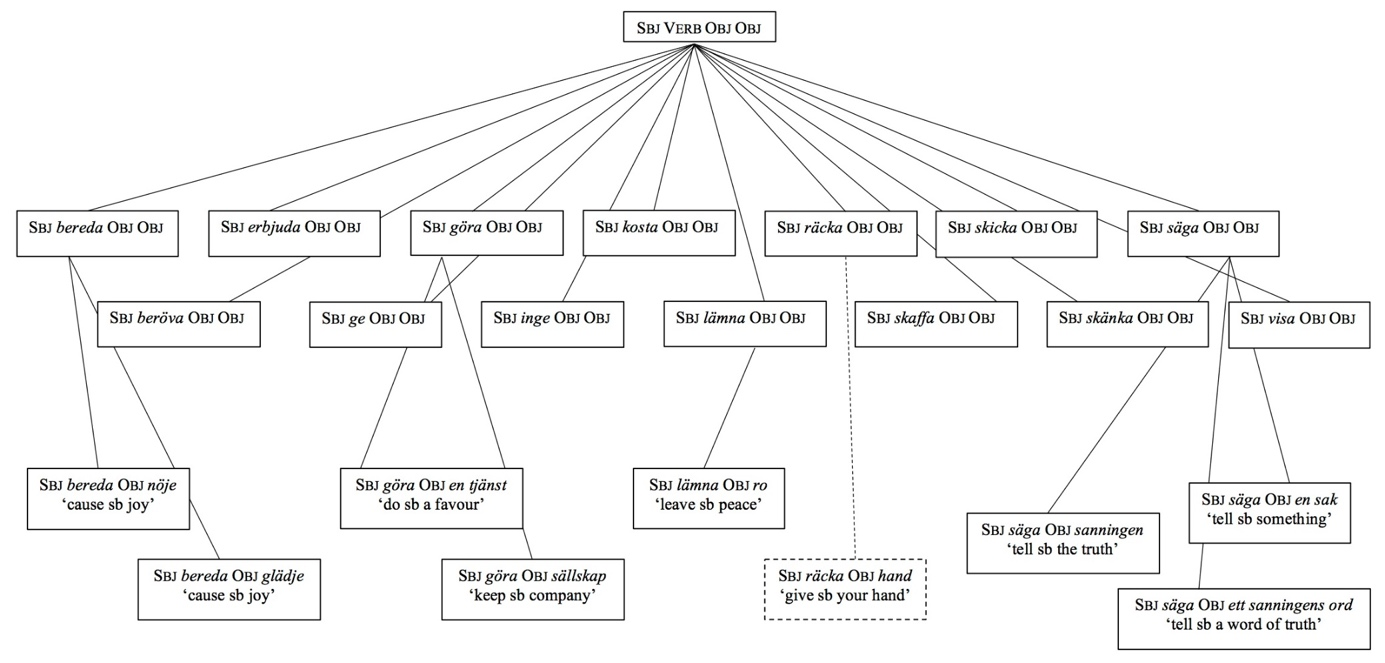
\includegraphics[width=\textwidth]{figures/a3-img002.jpg}
\caption{Taxonomic network of the DOC in present-day Swedish, including the most common verb-specific constructions as well as lexicalized expressions}
\label{fig:valdeson:4}

\begin{forest} for tree = {draw, grow' = 0}
[\textsc{Sbj Verb Obj Obj}
	[\textsc{Sbj} \textit{bereda} \textsc{Obj Obj}
		[\textsc{Sbj} \textit{bereda} \textsc{Obj} \textit{nöje}\\ 'cause sb joy']
		[\textsc{Sbj} \textit{bereda} \textsc{Obj} \textit{glädje}\\ 'cause sb joy']
	]
	[\textsc{Sbj} \textit{erbjuda} \textsc{Obj Obj}]
	[\textsc{Sbj} \textit{beröva} \textsc{Obj Obj}]
	[\textsc{Sbj} \textit{göra} \textsc{Obj Obj}
		[\textsc{Sbj} \textit{göra} \textsc{Obj} \textit{en tjänst} \\ 'do sb a favor']
		[\textsc{Sbj} \textit{göra} \textsc{Obj} \textit{sällskap} \\ 'keep sb company']
	]
	[\textsc{Sbj} \textit{ge} \textsc{Obj Obj}]
	[\textsc{Sbj} \textit{inge} \textsc{Obj Obj}]
	[\textsc{Sbj} \textit{kosta} \textsc{Obj Obj}]
	[\textsc{Sbj} \textit{lämna} \textsc{Obj Obj}
		[\textsc{Sbj} \textit{lämna} \textsc{Obj} \textit{ro} \\ 'leave sb peace']
	]
	[\textsc{Sbj} \textit{räcka} \textsc{Obj Obj}
		[\textsc{Sbj} \textit{räcka} \textsc{Obj} \textit{hand} \\ 'extend one's hand to sb', edge=dashed, dashed]
	]
	[\textsc{Sbj} \textit{skaffa} \textsc{Obj Obj}]
	[\textsc{Sbj} \textit{skicka} \textsc{Obj Obj}]
	[\textsc{Sbj} \textit{skänka} \textsc{Obj Obj}]
	[\textsc{Sbj} \textit{visa} \textsc{Obj Obj}]
	[\textsc{Sbj} \textit{säga} \textsc{Obj Obj}
		[\textsc{Sbj} \textit{säga} \textsc{Obj} \textit{sanningen} \\ 'tell sb the truth']
		[\textsc{Sbj} \textit{säga} \textsc{Obj} \textit{ett sanningens ord} \\ 'tell sb a word of truth']
		[\textsc{Sbj} \textit{säga} \textsc{Obj} \textit{en sak} \\ 'tell sb something']
	]
] 
\end{forest}


\end{figure}

\begin{sloppypar}
\figref{fig:valdeson:4} offers a proposal for a \isi{taxonomic network} of the \isi{double object construction} in \ili{Swedish}, covering different levels of schematicity. It is assumed that constructional knowledge is stored at both the topmost level and the verb-specific level. That the behaviour of the verb-specific constructions is not necessarily dependent on the topmost level is indicated by the divergent path of development found with the verb \textit{ge} ‘give’. The third level in the \isi{taxonomic hierarchy} shows the constructions that can be assumed to be stored as lexicalized expressions, i.e. constructions that are stored as fixed combinations of verb\,+\,\isi{direct object}. In this specific case, the network also illustrates the diachronic changes, since the lexicalized expressions with \textit{bereda} ‘cause’, \textit{göra} ‘make, do’, \textit{lämna} ‘hand’, and \textit{säga} ‘say, tell’ seem to have crystallized from the more schematic verb-specific mother constructions during the investigated period of 1800–1999. On the other hand, the \isi{lexicalized expression} \textit{räcka ngn handen} ‘extend one's hand to someone’ seems to be less entrenched in present-day \ili{Swedish} than in 19\textsuperscript{th} century \ili{Swedish}.
\end{sloppypar}


All the changes in the use of the DOC at various levels in the 19\textsuperscript{th} and 20\textsuperscript{th} centuries constitute different kinds of constructional changes. It should, however, be pointed out that the rather swift rate at which the changes have taken place might be partly due to the \isi{genre} of the studied texts. The language of written prose has changed quite substantially in \ili{Swedish} during the course of the 20\textsuperscript{th} century, in the direction of becoming more similar to the spoken language. It is quite possible that some of the changes identified in the current study are part of a larger change in the style of written prose in \ili{Swedish}, and that we are witnessing a combination of constructional and stylistic changes happening at the same time.


\section*{Acknowledgements}


I would like to thank the editors of this volume as well as three anonymous reviewers for their comments, which have considerably improved the quality of this paper.


\section*{Abbreviations}


DOC  \isi{Double object construction}


\section*{Sources}

\begin{description}
\item[Svensk prosafiktion] (`\ili{Swedish} prose fiction') 1800–1844. Available through \isi{Korp}.
\item[Svensk prosafiktion] (`\ili{Swedish} prose fiction') 1898–1901. Available through \isi{Korp}.
\item[Bonniersromaner I]   (`Bonnier novels I') 1976–1977. Available through \isi{Korp}.
\item[Bonniersromaner I]   (`Bonnier novels I') 1980–1981. Available through \isi{Korp}.
\item[Norstedsromaner]     (`Norstedts novels') 1999. Available through \isi{Korp}.
\end{description}

\section*{Electronic corpora}

\begin{description}
\item[\isi{Korp}:] \url{https://spraakbanken.gu.se/korp}
\end{description}

{\sloppy\printbibliography[heading=subbibliography,notkeyword=this]}
\end{document}
